\documentclass[11pt, a4paper, twoside]{tfg_dtic_upf}

% Languages
\usepackage[catalan,spanish,english]{babel}
\selectlanguage{english}

% Page margins (matches Word template ~2.5cm)
\usepackage{geometry}
\geometry{
  a4paper,
  top=2.5cm,
  bottom=2.5cm,
  inner=2.5cm,
  outer=2.5cm
}

% Graphics
\usepackage{graphicx}
\graphicspath{{figures/}}

% Font
\usepackage{times}

% No headings
\pagestyle{plain}

% Index
\usepackage{makeidx}
\makeindex

% Bibliography style (APA)
\bibliographystyle{apalike}

% Appendix
\usepackage{appendix}

% Math
\usepackage{amsmath}
\usepackage{amssymb}

% Tables
\usepackage{booktabs}
\usepackage{longtable}
\usepackage{multirow}

% Force figure placement
\usepackage{float}
\usepackage{placeins}

% Figures
\usepackage{subcaption}

% Units
\usepackage{siunitx}

% Fix chapter name to Catalan/Spanish style ("Chapter" → keep English for now)
% To match Word template: chapter number in smaller font, title in larger
% The cls already does: \huge "Chapter N" then \Huge TITLE — acceptable

% Hyperlinks (load last)
\usepackage[hidelinks]{hyperref}

% ============================================================
% THESIS METADATA
% ============================================================
\title{Population-Level Analysis of Post-Infarction Scar Geometry Using Standardised Polar Maps}
\author{Joan Company Company}
\thyear{Academic Year 2025--2026}
\supervisor{Prof.\ Oscar Camara Rey \\ Dr.\ Juli\`{a} Camps}
\grau{Grau en Enginyeria Matem\`{a}tica en Ci\`{e}ncia de Dades}

% ============================================================
\begin{document}

\frontmatter
\maketitle

% ============================================================
% DEDICATION (optional)
% ============================================================
\noindent [Dedication text here, or comment out this block]

\cleardoublepage

% ============================================================
% ACKNOWLEDGMENTS (optional)
% ============================================================
\noindent {\Large \sffamily Acknowledgments}

[Acknowledgment text here.]

\cleardoublepage

% ============================================================
% ABSTRACTS
% ============================================================
\selectlanguage{english}
\section*{\Large \sffamily Abstract}
[Abstract in English. Max 150 words.]

\selectlanguage{catalan}
\vspace*{\fill}
\section*{\Large \sffamily Resum}
[Resum en català. Màxim 150 paraules.]
\vspace*{\fill}

\selectlanguage{spanish}
\vspace*{\fill}
\section*{\Large \sffamily Resumen}
[Resumen en castellano. Máximo 150 palabras.]
\vspace*{\fill}

\selectlanguage{english}

\cleardoublepage

% ============================================================
% PREFACE (optional)
% ============================================================
{\bf Preface}

[Preface text here, or comment out this block.]

\cleardoublepage


\tableofcontents
\listoffigures
\addcontentsline{toc}{chapter}{List of Figures}
\listoftables
\addcontentsline{toc}{chapter}{List of Tables}

% ============================================================
% MAIN BODY
% ============================================================
\mainmatter

\chapter*{Introduction}
\addcontentsline{toc}{chapter}{Introduction}

[Introduction text. Context, motivation, research questions, thesis structure overview.]

\section*{Motivation}
[Why this work matters clinically and technically.]

\section*{Objectives}
\begin{enumerate}
    \item [Objective 1]
    \item [Objective 2]
    \item [Objective 3]
\end{enumerate}

\section*{Thesis Structure}
[Brief outline of chapters.]


\addcontentsline{toc}{part}{Methodology}

\chapter{Data and Cohort Description}

This chapter describes the clinical and imaging-derived dataset used throughout this project,
the selection criteria applied to obtain the analysis cohort, and the data structures available
for each patient case. All cases originate from the DEVELOP registry, a prospective
collection of post-myocardial infarction patients studied at Centro M\'{e}dico Teknon (Barcelona,
Spain) in the context of ventricular tachycardia (VT) risk assessment.

\section{The DEVELOP Registry and Clinical Context}

The source data consist of anonymised late gadolinium enhancement cardiac magnetic
resonance (LGE-CMR) studies from the DEVELOP registry. The original DICOM acquisitions
are stored in Teknon's internal storage system. The working dataset used in this project does
not operate directly on the DICOM files; instead, it uses the three-dimensional anatomical
and tissue meshes exported after post-processing. The dataset spans five acquisition years
(2021--2025), and the internal folder organisation within each year reflects the evolution of
the ADAS 3D export pipeline over time.

For each patient, image post-processing was carried out using ADAS 3D (Galgo Medical,
Barcelona), a software platform for three-dimensional cardiac image analysis. ADAS 3D
reconstructs the left ventricular (LV) shell from the LGE-CMR study and performs
semi-automatic tissue characterisation based on signal intensity. The software distinguishes
dense scar (core zone, CZ), heterogeneous peri-infarct tissue (border zone, BZ), and
healthy myocardium. The resulting surfaces are exported as VTK meshes, which constitute
the primary geometric input to the analyses in this work.

\section{Data Acquisition and Processing at Teknon}

Data extraction was performed on-site at Centro M\'{e}dico Teknon's computer system.
Building on prior familiarity with ADAS 3D acquired before the collaboration, the
understanding of the segmentation workflow was substantially deepened through direct
interaction with Teknon's technicians and clinicians: how scar appears under different
acquisition conditions, how tissue thresholds are adjusted, and how the resulting 3D models
relate to the underlying cardiac anatomy. Beyond the left ventricle, this experience also
provided exposure to left atrial ablation workflows and different arrhythmia types, including
atrial fibrillation and typical and atypical flutter.

Since no automatic pipeline existed for batch retrieval of specific mesh files from the ADAS
3D exports, a one-by-one extraction of CZ, BZ, healthy tissue, and corridor files was
undertaken for each patient. Version inconsistencies in file naming across acquisition years
(different ADAS 3D versions exported under DE-MRI, DE-MRI 3D, or DE-MRI 2D labels, and
the spelling variant TRANSMURABILITY for TRANSMURALITY) required the automated
loader to use pattern-based search rather than exact filenames.

The local dataset is organised as \texttt{/Basal/Data/LV/}. The automated scanner resolves
DE-MRI variants in order, locates anatomical meshes (Endo Layer, Epi Layer, Left
Ventricle, Myocardium), and searches the \texttt{LV/TISSUE/} subdirectory using ordered
glob patterns for core zone, border zone, healthy, scar, layer, and corridor files.

\section{Cohort Selection and Exclusion Criteria}

A case was considered valid only if it contained both a valid LV reconstruction directory and
a core zone mesh found inside \texttt{LV/TISSUE/}. An automated scan of the dataset was
performed across all patient folders.

Of the 168 total patient folders, 118 (70.2\%) contained a valid LV reconstruction directory,
and 105 (62.5\%) additionally contained a CZ mesh (Table~\ref{tab:cohort}). These 105
cases constitute the valid cohort. The 63 excluded cases fall into two categories: 50 lacked
an LV reconstruction directory entirely (35 had a \texttt{Basal/Data} path but no recognised
DE-MRI folder; 15 had no \texttt{Basal/Data} path), and 13 had an LV reconstruction but no
usable CZ mesh. The patient-level list of excluded cases is provided in Annex~\ref{app:supplementary}.

All 105 valid cases are used in the analyses presented in this work. No held-out split was
applied, as the primary objective is to build and evaluate a geometric representation rather
than to train a predictive model.

\begin{table}[htbp]
    \centering
    \caption{Cohort selection summary.}
    \label{tab:cohort}
    \begin{tabular}{lrr}
        \toprule
        Category & $n$ & \% \\
        \midrule
        Total patient folders & 168 & 100.0 \\
        With valid LV reconstruction & 118 & 70.2 \\
        With valid CZ mesh (analysis cohort) & 105 & 62.5 \\
        \midrule
        Excluded: no LV reconstruction directory & 50 & 29.8 \\
        \quad of which: Basal/Data present, no DE-MRI folder & 35 & --- \\
        \quad of which: no Basal/Data path & 15 & --- \\
        Excluded: LV present, no usable CZ mesh & 13 & 7.7 \\
        \bottomrule
    \end{tabular}
\end{table}

\section{Available Data per Patient}

Each valid case provides: (i) LV shell meshes representing the endocardial and epicardial
boundaries; (ii) tissue classification surfaces from ADAS 3D, primarily the core zone, with
additional border zone, healthy, and corridor meshes when available; (iii) transmural layer
meshes (Layer\_10 through Layer\_90), representing concentric wall-depth levels at 10\%
increments from the endocardial surface; and (iv) clinical metadata from the DEVELOP
registry CSV, including demographics, MRI-derived scar metrics, echocardiography,
arrhythmia variables, and follow-up outcomes. A detailed description of the clinical metadata fields and their completeness is provided in
Annex~\ref{app:supplementary}. The registry CSV is severely sparse outside MRI-derived
scar metrics: while LV mass, core zone, and border zone variables are available for
$\geq$96\% of registry entries, most demographic and clinical variables fall below 55\%
completeness, and outcome variables (dates of death, ablation, device implant) are available
for fewer than 6\% of entries. Sex information was available for 48 of the 105 valid patients,
with a predominantly male distribution consistent with the epidemiology of myocardial
infarction. Age was available for a subset of 48 patients (mean $63.0 \pm 11.5$ years). This
degree of missingness makes supervised clinical outcome modelling infeasible at the current
scale and motivates the use of the full cohort without clinical sub-grouping.

\section{Quality Control}

An automated three-dimensional rendering pipeline was implemented using PyVista. For
each case, the LV shell is displayed as a semi-transparent surface with the core zone
overlaid in opaque red from an isometric viewpoint. The resulting thumbnails were
assembled into a per-patient grid, enabling rapid visual inspection of segmentation
consistency, scar extent, and anatomical plausibility. This quality control step confirmed that
the 105 valid cases produce geometrically coherent scar representations suitable for
downstream analysis.

\begin{figure}[htbp]
    \centering
    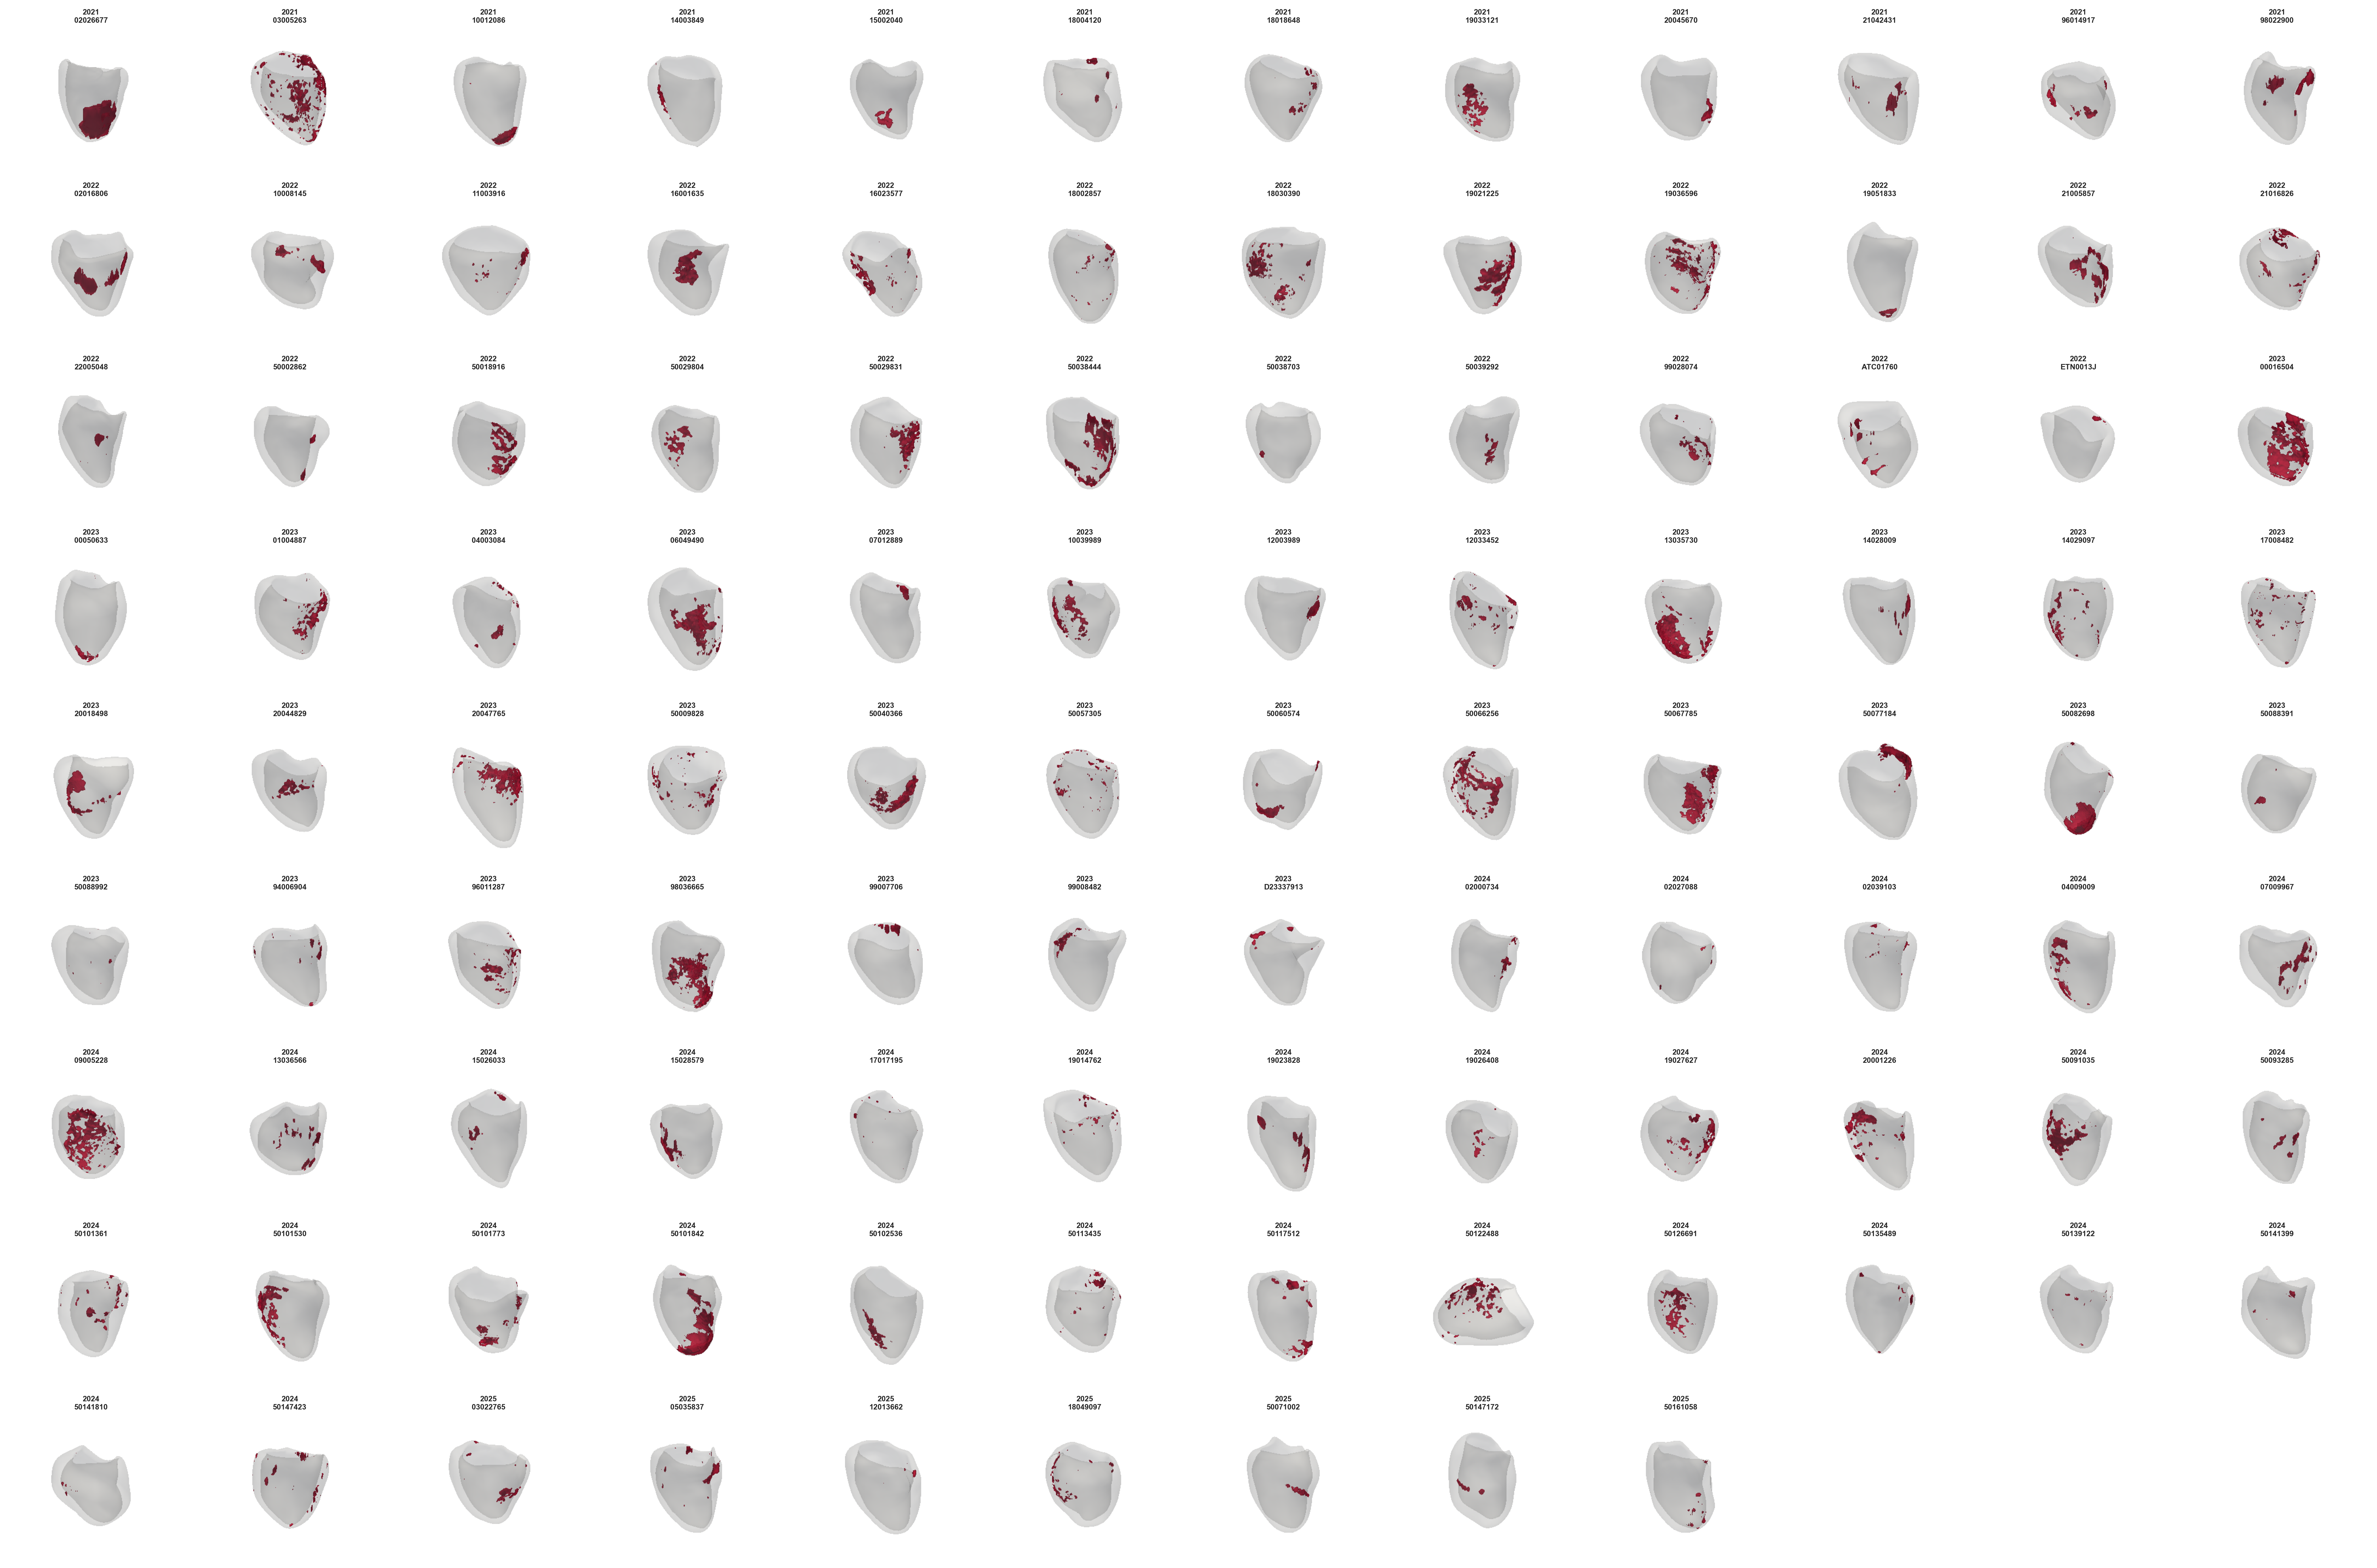
\includegraphics[width=\textwidth]{figures/3d_grid_full_cohort}
    \caption{QC grid of all 105 cases: LV shell (semi-transparent) with core-zone scar (red). Illustrates the cohort's wide range of scar extent, location, and morphology.}
    \label{fig:qc_grid}
\end{figure}

\label{chap:data}

\chapter{Polar Map Construction}

To enable population-level statistical analysis of post-infarction scar geometry, individual
three-dimensional scar surfaces must be projected onto a common two-dimensional
representation that preserves anatomical meaning across patients. This chapter describes
the pipeline that constructs this projection.

\section{Rationale: Why Flatten to 2D}

A statistical shape model of scar requires point-to-point correspondence across patients:
every patient's scar must be represented in a common coordinate frame so that
corresponding locations can be compared. An initial approach would be to establish this
correspondence directly on the three-dimensional LV surface, for instance by registering all
LV meshes to a common template and mapping scar labels through the deformation field.
However, exploratory analysis of the cohort revealed that post-infarction scar is extremely
variable in position, extent, and shape. Scar can appear in any coronary territory, at any
longitudinal level, and with transmural extent ranging from thin subendocardial ribbons to
full-thickness replacement.

A natural idea would have been to build the statistical shape model directly on the scar
tissue, treating each patient's scar as a surface. However, this proved impractical because
scar tissue presents highly heterogeneous three-dimensional morphologies across patients:
some infarctions produce concave apical geometries, others present flat surfaces, and yet
others exhibit convex or irregular shapes. This morphological diversity means that no single
reference scar shape exists onto which all patients could be mapped.

The bull's-eye or circumferential polar map provides a solution. By projecting the
three-dimensional LV surface onto a two-dimensional disk using cylindrical coordinates
anchored to the long axis and the septal reference, every patient's scar is expressed in the
same $(s, \theta)$ frame regardless of ventricular size, shape, or orientation. This
representation naturally provides inter-patient correspondence and reduces the problem to a
two-dimensional image amenable to standard statistical analysis.

\section{Apex Detection via Multi-Candidate Convex-Hull Search}

The apex is the geometric anchor of the entire polar map pipeline. Rather than relying on a
single principal component direction, the algorithm evaluates multiple candidate search
directions and selects the one that most clearly identifies the pointed apical tip of the left
ventricle.

The algorithm extracts the vertex coordinates of the full LV shell mesh and computes their
centroid. The centred point cloud is factored by singular value decomposition (SVD), yielding
principal components ordered by decreasing singular value. A separate SVD is performed
on the RV point cloud and its first principal component is also extracted. These three
directions---LV PC1, LV PC2, and RV PC1---form the list of candidate search directions.

For each candidate direction $\mathbf{a}$, let $\mathbf{c}$ denote the LV centroid and
$P_\text{hull}$ the set of convex-hull vertices. Each hull vertex $\mathbf{p}_i$ is projected
onto the candidate direction relative to the centroid, yielding a signed scalar distance
$d_i = (\mathbf{p}_i - \mathbf{c}) \cdot \mathbf{a}$. The apex candidate is the hull vertex
with the largest absolute projection. To score how pointed this candidate is, a half-span $H$
is computed from the full vertex set: $H = (d_\text{max} - d_\text{min}) / 2$. The
eccentricity is then $e = |d_\text{apex}| / H$. The candidate direction yielding the highest
eccentricity is selected.

LV PC1 captures the apex-to-base elongation in the majority of cases. However, pathological
ventricular remodelling or mesh truncation can make the LV point cloud nearly isotropic,
causing PC1 to align with circumferential rather than longitudinal variance. RV PC1 is
included because the RV's strongly elongated crescent shape reliably recovers the
base-to-apex direction even when the LV shape is unfavourable. LV PC2 provides an
additional fallback for the rarer cases where the true long axis is captured by the second
rather than the first principal direction.

\section{Long-Axis and Septal Reference}

Once the apex has been detected, the long axis is constructed as the unit vector pointing
from the detected apex toward the LV centroid. This construction guarantees that the axis
passes through the apex by definition, that the direction is unambiguously from apex toward
base, and that the result is entirely LV-intrinsic regardless of which search direction found the
apex.

A circumferential zero-angle must be established so that the anterior, septal, inferior, and
lateral walls map to consistent angular positions across patients. The septal direction is
computed from the spatial relationship between the LV and RV centroids, both restricted to a
basal band spanning 50 to 90 percent of the apex-to-base distance to avoid bias from the
apically-extending RV free wall. The raw direction vector from the LV centroid to the RV
centroid is projected onto the plane perpendicular to the long axis and normalised to a unit
vector.

\section{Polar Coordinate Computation}

Every point on the LV surface is mapped to two cylindrical polar coordinates. The
longitudinal coordinate $s$ is obtained by projecting the displacement from the apex onto the
long axis and normalising by the total span, so that $s = 0$ at the apex and $s = 1$ at the base:
\begin{equation}
    s = \frac{(\mathbf{p} - \mathbf{apex}) \cdot \mathbf{axis}}{\text{span}}.
    \label{eq:longcoord}
\end{equation}
The circumferential angle $\theta$ is measured relative to the septal reference direction. The
continuous coordinates are discretised into a $64 \times 128$ (radial $\times$ angular) grid,
giving approximately 6 vertices per bin for a typical LV shell mesh of ${\sim}50{,}000$ vertices.

The bull's-eye grid is partitioned into the AHA 17-segment model \cite{cerqueira2002} using four concentric rings:
the apical cap ($s \in [0, 0.25]$, segment 17), the apical ring ($s \in [0.25, 0.50]$, four
$90^{\circ}$ sectors), the mid-cavity ring ($s \in [0.50, 0.75]$, six $60^{\circ}$ sectors), and
the basal ring ($s \in [0.75, 1.00]$, six $60^{\circ}$ sectors).

\begin{figure}[htbp]
    \centering
    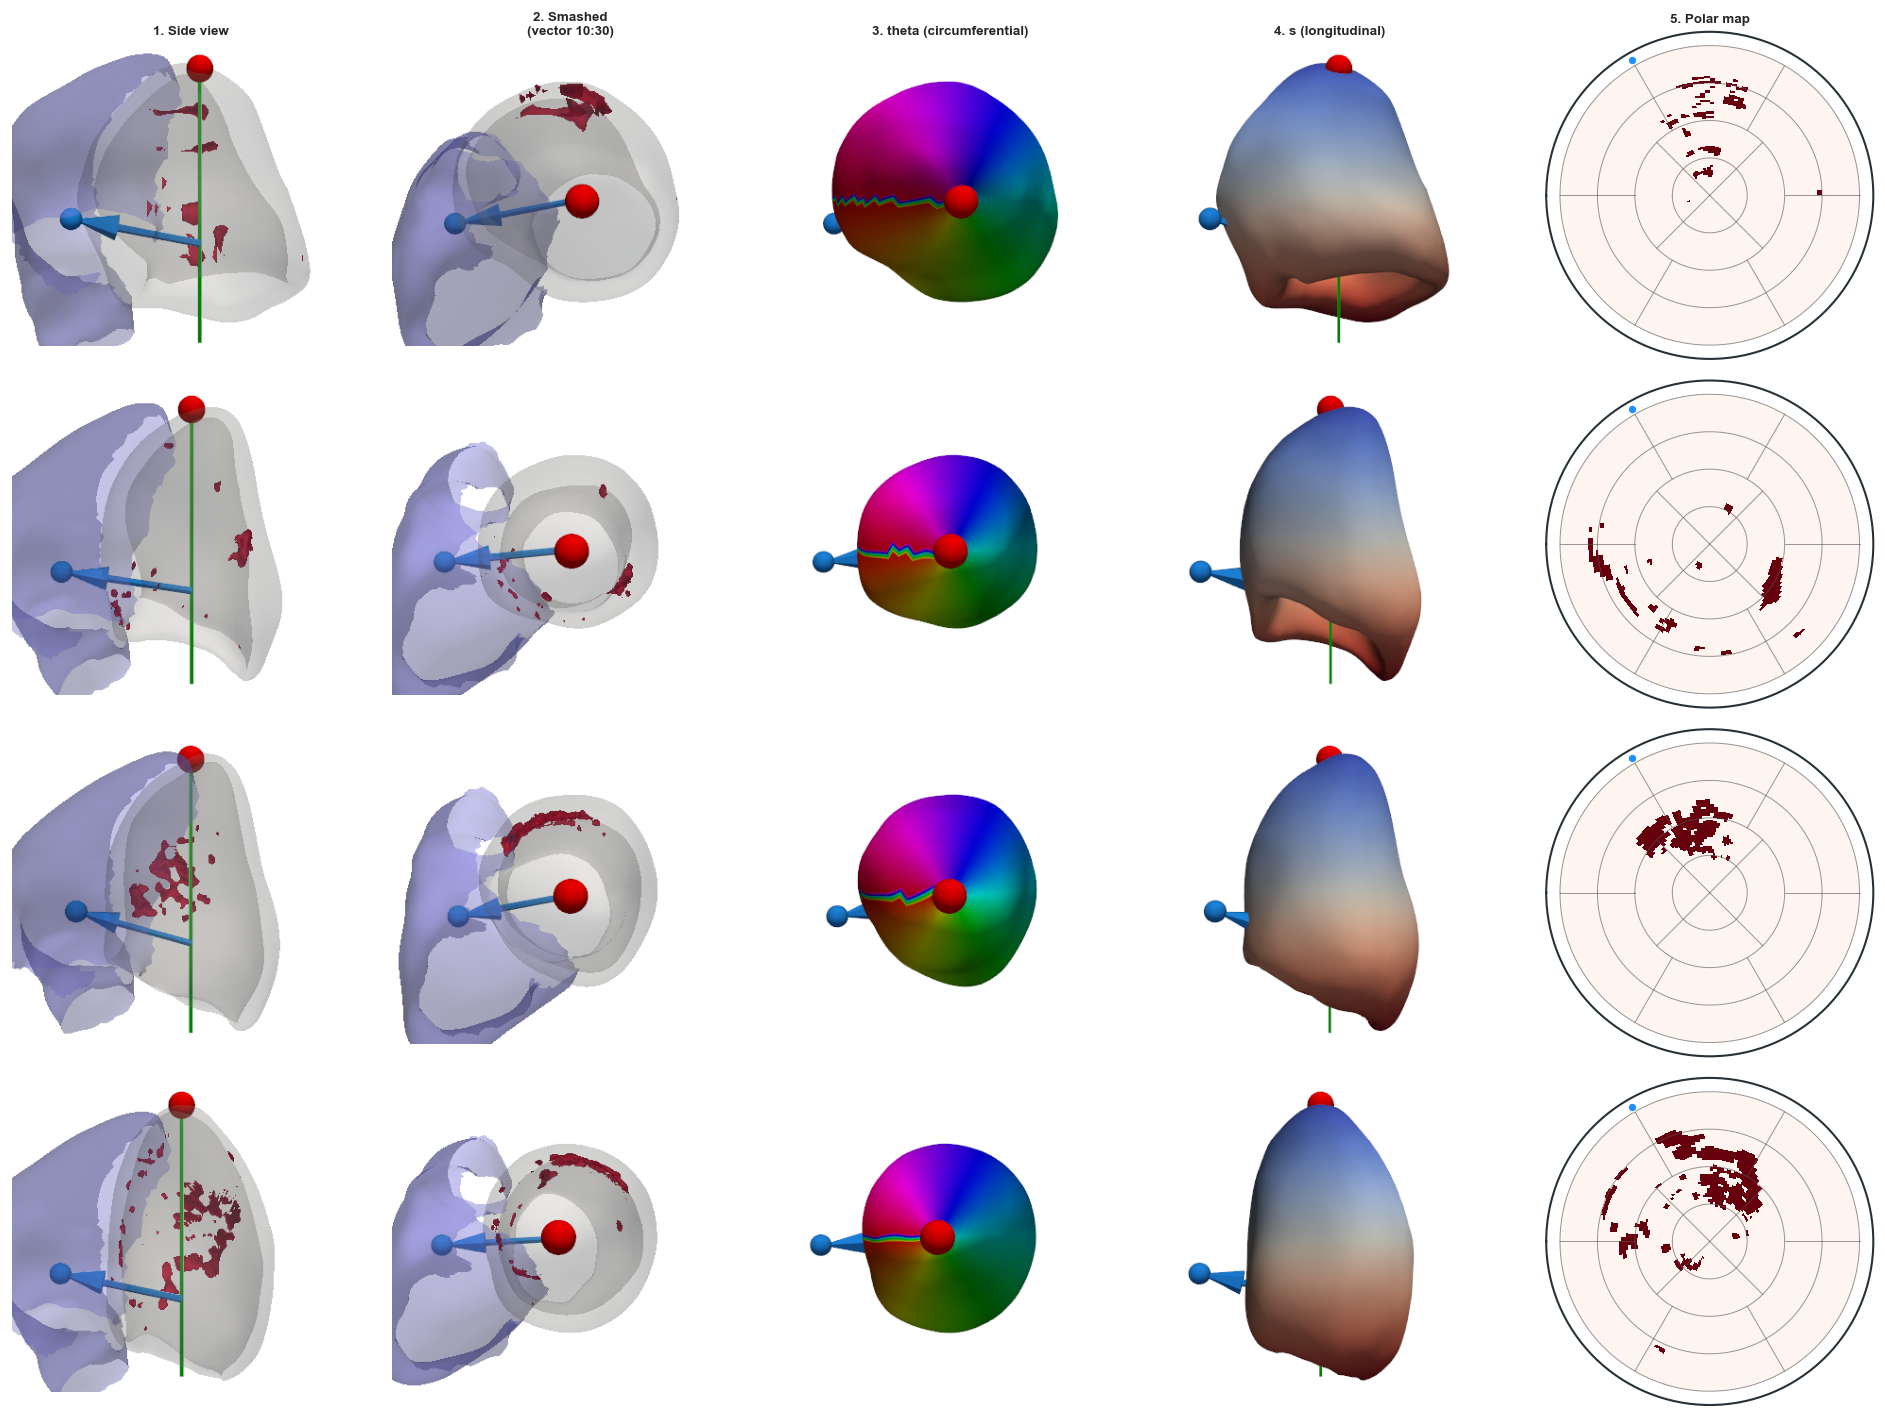
\includegraphics[width=\textwidth]{figures/polar_map_steps}
    \caption{Polar map projection pipeline. From left to right: original 3D LV and RV meshes; long-axis detection and apex-down re-orientation; longitudinal coordinate $s$ computed apex-to-base; circumferential angle $\theta$ anchored to the septal reference; final 2D bull's-eye polar map with AHA 17-segment overlay.}
    \label{fig:polarmaps2}
\end{figure}

\section{Scar Projection Methods}

Three complementary methods are used to project scar onto the polar grid. The
\textbf{vertex-based method} assigns a binary label to each polar bin: a bin is marked as
scarred if at least one core-zone vertex projects into it. When averaged across patients, each
grid value represents the fraction of patients with scar in that location. This method is the
primary representation because it is reversible (supports round-trip 3D$\to$2D$\to$3D
mapping), separates location from intensity, and transfers cleanly to target meshes with
different vertex densities.

The \textbf{area-based method} accumulates triangle surface areas per bin (mm$^2$),
capturing absolute scar burden. The \textbf{coverage method} divides CZ area by total LV
area per bin, removing bin-size and LV-size bias. Consistency between all three approaches
was verified to ensure that findings are not artefacts of the binary representation.

\section{Polar Map Verification}

To provide an independent qualitative assessment of anatomical plausibility, the polar maps
produced by the proposed pipeline were compared against those generated by the
conformal flattening method of N\'{u}\~{n}ez Garc\'{i}a \cite{nunez2018} for four representative cases. Both methods
operated on the same Endo Layer mesh, which is required as input by the reference
flattening script; the main pipeline uses the full LV shell for axis and span estimation in all
other analyses, and this difference introduces a small systematic variation in longitudinal
span that is independent of the comparison's primary findings.

One methodological difference concerns scar detection: the proposed method projects Core
Surface vertices directly onto the polar grid, whereas the reference method proximity-labels
endocardial surface points within a tolerance derived from the Core Surface mesh spacing,
then maps those labelled points using the 2D flat coordinates. A further distinction concerns
the radial mapping: the reference method applies a radial displacement transform of the form
$r_\text{new} = r^{1/3}$ to the conformally flattened disk \cite{paun2017}, which
redistributes points outward and produces denser coverage near the basal ring. The
proposed pipeline uses a linear longitudinal mapping and therefore does not exhibit this
redistribution. Prior to visual comparison, both polar maps were aligned to the same septal
reference direction.

\label{chap:polarmaps}

\chapter{Statistical Characterisation of Scar}

\section{AHA-17 Segmentation, Territory Assignment, and Normality Diagnostics}

Scar burden per segment was defined as the fraction of polar-map bins classified as
scar-positive. Territory burden was defined analogously over LAD (segments 1, 2, 7, 8, 13,
14, 17; 4\,448 bins, 54.3\%), RCA (segments 3, 4, 9, 10, 15; 1\,888 bins, 23.0\%), and LCX
(segments 5, 6, 11, 12, 16; 1\,856 bins, 22.7\%). A territory was considered involved when
at least 2\% of its polar bins were scar-positive. This threshold was selected via sensitivity
analysis across candidate values (1\%, 2\%, 3\%, 5\%, 10\%); the full sensitivity curve is
shown in Figure~\ref{fig:app_territory_threshold} in the Appendix. At 1\% the multi-territory
fraction exceeded 60\%, implausibly high for a focal-infarct cohort; thresholds above 3\%
progressively assigned no-scar classification to patients with minor genuine involvement.
The 2\% value represents the earliest stable point at which single-territory classification
reaches its plateau and the no-scar fraction remains low (${\sim}10\%$).

Prior to selecting inferential methods, the distributional properties of all analysis variables
were assessed using quantile--quantile plots and chi-squared goodness-of-fit plots. Of all
variables examined, only age satisfied the normality criterion; all scar-related variables
showed strong zero-inflation and right skewness. All subsequent analyses therefore relied on
non-parametric methods and resampling-based confidence intervals.

Table~\ref{tab:aha17summary} reports prevalence and conditional extent for all 17 AHA segments.

\begin{table}[htbp]
    \centering
    \caption{AHA 17-segment scar burden summary ($n=105$). Segments ordered by ring (basal, mid, apical, apex). Extent = fraction of polar-map bins classified as scar-positive.}
    \label{tab:aha17summary}
    \small
    \begin{tabular}{rllrrrr}
        \toprule
        Seg & Label & Ring & Prev.\ (\%) & Mean (all) & Mean (pos.) & Median (pos.) \\
        \midrule
        1  & Bas ant      & Basal & 30.5 & 0.023 & 0.077 & 0.044 \\
        2  & Bas ant-sep  & Basal & 37.1 & 0.023 & 0.061 & 0.039 \\
        3  & Bas inf-sep  & Basal & 23.8 & 0.014 & 0.059 & 0.030 \\
        4  & Bas inf      & Basal & 33.3 & 0.014 & 0.041 & 0.026 \\
        5  & Bas inf-lat  & Basal & 44.8 & 0.032 & 0.071 & 0.033 \\
        6  & Bas ant-lat  & Basal & 39.0 & 0.032 & 0.083 & 0.063 \\
        \midrule
        7  & Mid ant      & Mid   & 34.3 & 0.042 & 0.121 & 0.048 \\
        8  & Mid ant-sep  & Mid   & 48.6 & 0.057 & 0.117 & 0.063 \\
        9  & Mid inf-sep  & Mid   & 52.4 & 0.060 & 0.114 & 0.060 \\
        10 & Mid inf      & Mid   & 61.0 & 0.088 & 0.145 & 0.080 \\
        11 & Mid inf-lat  & Mid   & 56.2 & 0.100 & 0.178 & 0.110 \\
        12 & Mid ant-lat  & Mid   & 46.7 & 0.063 & 0.136 & 0.071 \\
        \midrule
        13 & Api ant      & Apical & 41.0 & 0.060 & 0.148 & 0.066 \\
        14 & Api sep      & Apical & 41.0 & 0.078 & 0.190 & 0.098 \\
        15 & Api inf      & Apical & 56.2 & 0.058 & 0.103 & 0.059 \\
        16 & Api lat      & Apical & 49.5 & 0.051 & 0.103 & 0.059 \\
        \midrule
        17 & Apex         & Apex  & 53.3 & 0.052 & 0.097 & 0.024 \\
        \bottomrule
    \end{tabular}
\end{table}

\section{Within-Patient Spatial Tests and Bootstrap Confidence Intervals}

Whether scar burden varies systematically across AHA segments within the same patient
was tested using the Friedman test, a non-parametric analogue of one-way
repeated-measures ANOVA. Each of the 105 patients contributed a vector of 17 paired
segment-burden values. Pairwise post-hoc comparisons were conducted using Wilcoxon
signed-rank tests with Bonferroni correction for the 136 pairwise comparisons.

Population-level confidence intervals for the mean scar burden in each AHA segment were
estimated via patient-level bootstrap resampling. In each of 2\,000 iterations, 105 patients
were sampled with replacement---preserving each patient's full 17-segment vector---and the
mean burden per segment was recomputed. The 2.5th and 97.5th percentiles defined the
95\% confidence interval. The primary purpose of this procedure is not to establish
statistical significance of individual segment means, but to quantify the uncertainty around
population estimates for the atlas and archetype maps. Because the underlying distributions
are zero-inflated and heavily skewed, symmetric normal-theory intervals would systematically
misrepresent the sampling distribution: they produce symmetric error bars around means
that are, in reality, bounded below by zero and pulled by long positive tails. The bootstrap
intervals are asymmetric by construction and therefore faithfully reflect the shape of the
sampling distribution, providing honest uncertainty bounds for the population scar atlas.

\section{Age and Sex Associations}

Association between age and segment-level scar burden was assessed using Spearman
rank correlation in the 48 patients with available age labels (mean age $63.0 \pm 11.5$
years). Bonferroni correction was applied across the 17 segments, yielding an adjusted
significance threshold of $\alpha = 0.05/17 = 0.0029$. Sex-stratified analysis was limited by
severe label imbalance (38 male, 10 female among patients with sex information).

\section{Dimensionality Reduction and Correlation Structure}

PCA was applied to the 17-dimensional scar-burden vectors after $z$-score standardisation
(zero mean, unit variance per segment). The aim was to identify the dominant spatial modes
of scar variability and assess the intrinsic dimensionality of the scar-pattern space.
Component loadings were mapped back onto the AHA bullseye representation to visualise
the spatial scar phenotype associated with each PC.

Two correlation analyses complement the PCA. First, the inter-segment correlation matrix
computes Spearman rank correlations between all $17 \times 17$ pairs of AHA segment
burdens across patients. Second, the territory burden correlation matrix
computes the $3 \times 3$ Spearman correlation matrix between LAD, RCA, and LCX burden.
This determines whether territory burdens are effectively independent dimensions---weak
correlations would support treating territories as orthogonal axes of scar phenotype---or
whether multi-territory involvement is the norm, implying that a single ``core zone burden''
scalar captures most of the territory-level information.

\section{Population Variability and Archetype Maps}

Population variability maps were computed across the polar maps. Archetype maps were
constructed by grouping patients according to their dominant coronary territory and
computing the mean polar map within each group. Ring-level and territory-level coverage
summaries, bootstrap confidence intervals, and variability maps were recomputed using the
area-based and coverage projections.

\section{Transmurality: Continuous Vertex-Depth Computation}

The analyses above characterise scar extent on the LV surface but do not capture how
deeply scar penetrates through the ventricular wall. Transmurality---the fraction of wall
thickness affected by scar---is clinically important because transmural scar has different
electrophysiological consequences than subendocardial scar.

An initial approach used the nine layer-specific scar meshes exported by ADAS 3D
(Layer\_10 through Layer\_90), projecting each layer mesh onto the $64 \times 128$ polar
grid and computing onset and elongation as the shallowest and span of scar-containing
layers. However, the discrete layer resolution proved too coarse: the resulting transmurality
values were nearly uniform across the cohort, with insufficient variation to differentiate scar
profiles meaningfully.

To overcome this limitation, a continuous vertex-depth approach was developed. For each
patient, the endocardial and epicardial surfaces of the LV wall are loaded, and a cKDTree
spatial index is built for each. Every vertex of the core-zone scar mesh is then located in 3D
space, and its Euclidean distances to the nearest point on the endocardial surface ($d_\text{endo}$)
and the epicardial surface ($d_\text{epi}$) are computed. The fractional wall depth of that vertex
is defined as:
\begin{equation}
    \text{depth\_frac} = \frac{d_\text{endo}}{d_\text{endo} + d_\text{epi}}.
    \label{eq:depthfrac}
\end{equation}
This yields a continuous value in $[0, 1]$, where 0 represents the endocardial wall and 1 the
epicardial wall. Each scar vertex is then projected onto the same $64 \times 128$ polar grid
used for the binary scar maps. Within each polar bin, the minimum depth fraction across all
scar vertices falling into that bin defines the \emph{onset} (the shallowest wall depth at which
scar begins), and the maximum depth fraction defines the \emph{outermost depth}.
Transmurality per bin is then computed as:
\begin{equation}
    \text{transmurality} = \text{outermost\_depth} - \text{onset}.
    \label{eq:transmurality}
\end{equation}

These bin-level values are aggregated at three levels (segment, territory, and fragment) over
scar-positive bins only; the aggregation procedure is detailed in
Appendix~\ref{app:transmuralagg}. This decomposition distinguishes three clinically
relevant scar profiles: thin subendocardial (low onset, low transmurality), transmural (low
onset, high transmurality), and midwall (high onset, variable transmurality).

\section{Fragment-Level Characterisation}
\label{sec:fragments}

Connected-component labelling was applied to each patient's 3D core-zone mesh to identify
spatially distinct scar fragments (minimum 50 vertices). Each fragment is projected to the
polar grid and assigned to a ring zone (apex, apical, mid, basal) by its centroid row and to a
coronary territory by plurality vote across its polar bins. For each fragment, the mean onset,
mean outermost depth, and mean transmurality are computed from the continuous
vertex-depth grids over the fragment's polar footprint. Fragment size (number of polar bins),
ring position, and territory assignment complete the per-fragment descriptor set.

\section{Within-Patient Consistency Between Extent and Transmurality}

For each patient, the 17-element segment-level extent vector (fraction of bins that are
scar-positive per AHA segment) is correlated with the 17-element per-segment mean
transmurality vector (mean transmurality over scar-positive bins in each segment) using
Spearman rank correlation. Values near zero indicate that extent and transmurality carry
independent information about the scar phenotype---a patient may have extensive but
shallow scar, or focal but deeply penetrating scar---and that both descriptors are needed.
Values near $+1$ indicate redundancy, where one measure largely substitutes for the other.

\section{Transmurality Gradient Within Fragments}

For each 2D polar-map fragment with at least 20 bins, each bin is classified as \emph{core}
(three or more scar-positive 4-connected neighbours) or \emph{edge} (fewer than three).
The fragment gradient is then defined as the difference between the mean transmurality of
core bins and the mean transmurality of edge bins. A positive population-mean gradient
indicates that scar has a dense-core / thin-edge transmural structure, which is relevant for
arrhythmogenesis because the gradient zone---where transmurality transitions from thick to
thin---is precisely where conduction slows and re-entry circuits may form.

\section{Geometric Shape Descriptors}

Four additional per-patient descriptors capture aspects of scar geometry not encoded in
segment-level or transmurality analyses. \textbf{Circumferential extent} is the fraction of
angular columns containing at least one scar-positive bin per ring level (apex, apical, mid,
basal), quantifying tangential spread around the ventricular wall. \textbf{Scar compactness}
is $4\pi \cdot \text{area}/\text{perimeter}^2$ of the largest 2D connected component (1 for
a perfect circle, lower for elongated or irregular shapes), supplemented by aspect ratio and
fragment count; these metrics are independent of total scar burden and capture whether scar
forms a single compact lesion or a fragmented pattern. \textbf{Endocardial--epicardial
dominance} classifies each scar-positive bin by onset depth: endocardial ($\leq 30\%$),
midwall (30--60\%), or epicardial ($> 60\%$ of wall thickness), distinguishing ischaemic
from non-ischaemic onset patterns. \textbf{Apex-to-base gradient} fits a first-order
polynomial to row-level mean burden ($s \in [0,1]$, apex to base), with Spearman
correlation as a non-parametric summary of longitudinal scar organisation.

\label{chap:statistical}

\chapter{Retrieval-Based Scar Generation}

The previous chapters established a compact geometric characterization of post-infarction
scar. This chapter presents a retrieval-based generation (RBG) framework that leverages
these descriptors to retrieve plausible scar patterns from the available patient cohort.

\section{Problem Formulation}

Given a target specification---which may be a partial clinical profile, a set of desired scar
properties, or an existing patient to be matched---the goal is to produce a plausible scar
polar map that is consistent with the population-level distribution observed in real data.
Formally, given a query vector $\mathbf{q} \in \mathbb{R}^d$ encoding the desired scar
characteristics, the system must return one or more polar maps drawn from real observations
whose descriptor vectors are close to $\mathbf{q}$.

A retrieval-based strategy was chosen over generative alternatives such as VAEs, GANs, or
diffusion models for three main reasons. First, the available cohort is relatively small for
training deep generative models with high-dimensional outputs. Second, every output is, by
construction, a real patient scar observed in clinical practice, which provides a strong
plausibility constraint. Third, retrieval is fully interpretable: the distance to the nearest
neighbour quantifies how well the query is represented in the case base, and the identity and
geometry of the retrieved patient can be inspected directly. The main limitation is that the
method cannot synthesize completely new scar shapes outside the observed cohort; this is
partially addressed through probabilistic retrieval.

\section{Scar Descriptor Space}

The retrieval engine operates in a descriptor space where each patient is represented by a
fixed-length feature vector $\mathbf{v} \in \mathbb{R}^d$. Six candidate descriptor vectors
were compared, designed to evaluate the relative contribution of structured scar features,
AHA segment burdens, dimensionality reduction, and pixel-level polar-map information.

The \textbf{full} vector (39 features) contains all structured descriptors: segment-level scar
burden across the 17 AHA segments, coronary territory fractions, number of involved
territories, circumferential spread, compactness, apex-to-base gradient, number of
fragments, and fragment-level radial and size descriptors. The \textbf{full\_no\_seg} variant
(22 features) removes the 17 AHA segment burdens to test whether territory, morphology,
and fragment descriptors are sufficient without per-segment information. Pruned variants
were derived using SVD contribution analysis: features with contributions below the 25th
percentile were dropped, yielding \textbf{full\_pruned} (29 features) from the full vector and
\textbf{full\_ns\_pruned} (16 features) from the segment-free variant. The
\textbf{pmap\_only} vector (8 features) uses PCA scores from the flattened binary polar
maps, capturing pixel-level spatial variation without manually designed features. The
\textbf{full\_ns+pmap} hybrid (30 features) combines the non-segment structured features
with the polar-map PCA scores.

\section{Similarity Metric and Retrieval Strategy}

Three distance metrics were evaluated on the selected descriptor: standard Euclidean,
Manhattan, and cosine. Manhattan distance on $z$-score normalised features was selected
as the primary metric based on leave-one-out performance.

The retrieval engine follows a $k$-nearest-neighbour strategy. Two modes were implemented:

\textbf{Deterministic retrieval} ($k = 1$) returns the single nearest neighbour:
$i^* = \arg\min_i\, d(\mathbf{q}, \mathbf{v}_i)$.
This mode maximises descriptor-space similarity but always returns the same patient for the
same query.

\textbf{Probabilistic retrieval} ($k = 10$) retains the top 10 neighbours and samples
according to softmax weights:
\begin{equation}
    p_i = \frac{\exp(-d_i/\tau)}{\sum_j \exp(-d_j/\tau)},
    \label{eq:softmax}
\end{equation}
where $\tau > 0$ is a temperature parameter controlling the sharpness of the distribution:
as $\tau \to 0$ all weight concentrates on the nearest neighbour (recovering deterministic
retrieval), while larger $\tau$ spreads weight more uniformly across the top-$k$ candidates,
increasing diversity at the cost of similarity. A value of $\tau = 1.0$ was used throughout:
probabilistic experiments showed that even at this setting the softmax weights were already
strongly concentrated on the nearest neighbour for most patients, leaving very little
probability mass on non-close cases; a smaller $\tau$ would have further reduced diversity
without meaningful gain in retrieval quality. Every output remains a real patient scar,
but repeated calls with the same query can return different plausible cases.

\section{Evaluation Framework}

Retrieval quality was assessed using leave-one-out cross-validation across the full cohort.
For each patient, that patient was temporarily removed from the case base and used as the
query. Three complementary metrics were computed: scar amount error $|\Delta\text{CZ}|$
(absolute difference in core-zone burden between target and retrieved patient), segment
Dice (binarised overlap over the AHA 17-segment model), and polar-map Dice (pixel-level
overlap on the $64 \times 128$ polar grid). All six candidate vectors were evaluated using this
protocol with the same distance metric.

% Figure removed per revision.

\label{chap:retrieval}

\addcontentsline{toc}{part}{Results, Discussion and Conclusions}

\chapter{Results}
\label{chap:results}

\section{Cohort and Data Availability}

This section describes cohort composition, scar morphology heterogeneity across the
105 valid cases, and available clinical metadata.

\subsection{Scar morphology and inter-patient heterogeneity}
\label{sec:scarmorph}

Visual inspection of the full-cohort 3D grid confirmed that all 105 cases produce
geometrically coherent LV reconstructions with identifiable core-zone surfaces. Beyond
confirming quality, the grid reveals the amplitude of scar morphology present in this cohort.
Scar extent ranges from small, focal lesions occupying a single wall segment to large,
multi-territory scars covering a substantial fraction of the myocardium. Spatial organisation
varies from compact, contiguous surfaces to fragmented geometries with disconnected
components distributed across different wall regions. Infarction location spans all three coronary territories (LAD, RCA, LCX)---with scar
affecting inferior, anterior, lateral, and septal walls---at basal, mid-ventricular, and
apical levels, with variable wall-depth involvement from subendocardial to near-transmural.
This degree of heterogeneity is a defining characteristic of the cohort and directly motivates
the need for a shape representation that makes no assumptions about scar location, extent,
or connectivity.

\subsection{Clinical metadata and demographic profile}

Cross-referencing the DEVELOP registry CSV (173 records, 88 with segmentation flag) with
the geometrically valid cases yields 48 patients with usable age and sex labels. Among
these, 38 are male (79.2\%), mean age $63.0 \pm 11.5$ years (median 63.0, IQR 54.8--72.0).
The high missingness of demographic and outcome variables makes supervised clinical
outcome modelling infeasible; all geometric analyses proceed on the full 105-case cohort.

\section{Polar Map Construction and Orientation Verification}

This section reports pipeline performance across the 105-case cohort: apex detection
outcomes, projection method consistency, grid resolution sensitivity, and comparison
against a reference flattening method.

\subsection{Apex and axis detection}

The multi-candidate apex detection strategy (Section~\ref{sec:polarmaps}) was applied
to all 105 cases. LV~PC1 was selected as the apex-defining direction in 74\% of cases,
RV~PC1 in 21\%, and LV~PC2 in the remaining 5\% (Figure~\ref{fig:apexdirection}). In
the RV~PC1 cases, LV~PC1 aligned with circumferential rather than longitudinal variance,
producing an incorrect apex location shifted toward the lateral wall (the free wall of the
left ventricle facing away from the septum, in the direction opposite to the right ventricle). In the LV~PC2 cases,
near-equal variance in the two largest dimensions caused the true long axis to be captured
by the second rather than the first principal direction. The multi-candidate strategy correctly
identified the apical tip in all 105 cases.

A forced-LV-PC1 ablation confirmed that constraining the axis to LV~PC1 regardless of
eccentricity produces incorrect apex detection in the 25\% of cases where RV~PC1 or
LV~PC2 would otherwise be selected, demonstrating that a single fixed direction is
insufficient for this cohort (Figure~\ref{fig:app_axis_winner} in Appendix). A qualitative
comparison against the reference flattening method of N\'{u}\~{n}ez Garc\'{i}a
\cite{nunez2018} is presented in Section~\ref{sec:polarmapverif}.

\begin{figure}[ht]
    \centering
    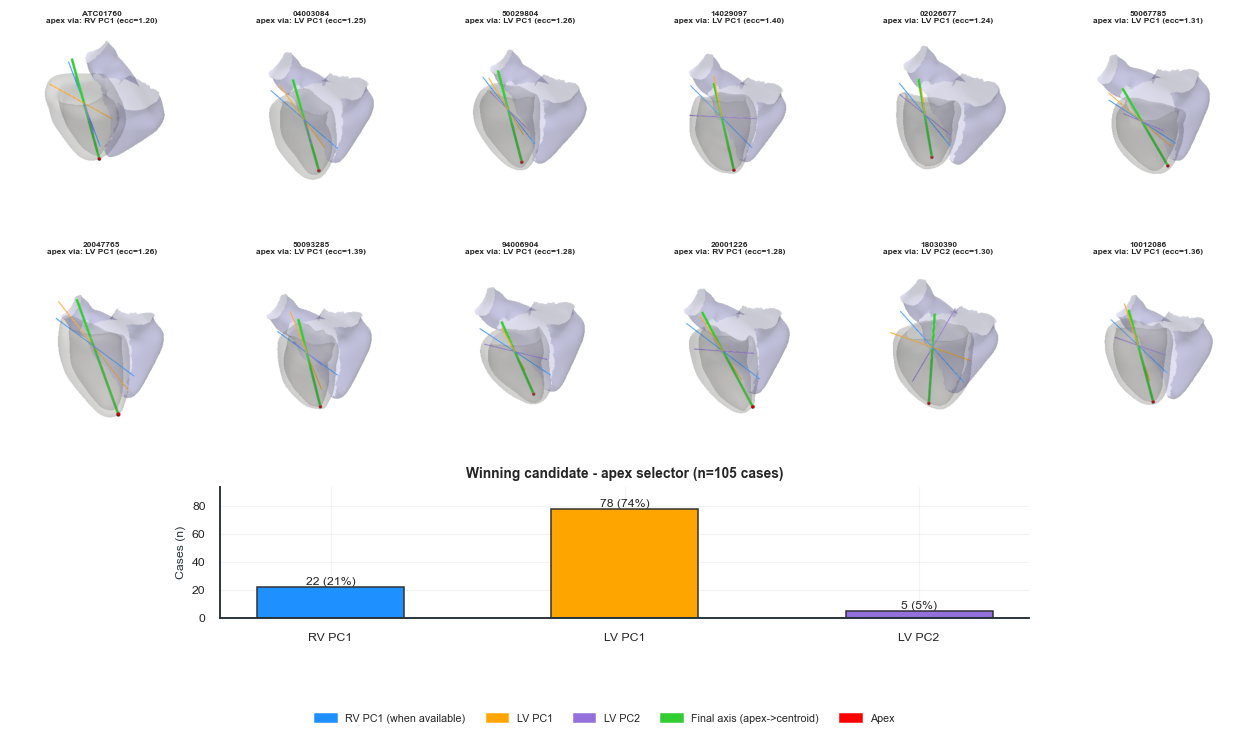
\includegraphics[width=0.68\textwidth]{figures/d6_long_axis_candidates}
    \caption{Apex-defining direction selected per patient ($n=105$): LV~PC1 in 74\%, RV~PC1 in 21\%, LV~PC2 in 5\%.}
    \label{fig:apexdirection}
\end{figure}

\vspace{-0.8em}
\subsection{Projection method comparison}
\label{sec:projmethods}

Three complementary projection methods were evaluated at the population level: the
vertex-based method (binary scar presence per polar bin), the area-based method
(projected core-zone surface area in mm$^2$ per bin), and the coverage method
(core-zone area divided by total LV area per bin). The spatial pattern of scar concentration is consistent across methods: all three identify
the same high-burden regions and the same low-burden regions, with differences confined
to relative intensity rather than spatial location. Population-level superposition maps for
all three methods are shown in Figure~\ref{fig:superposition}.

\begin{figure}[H]
    \centering
    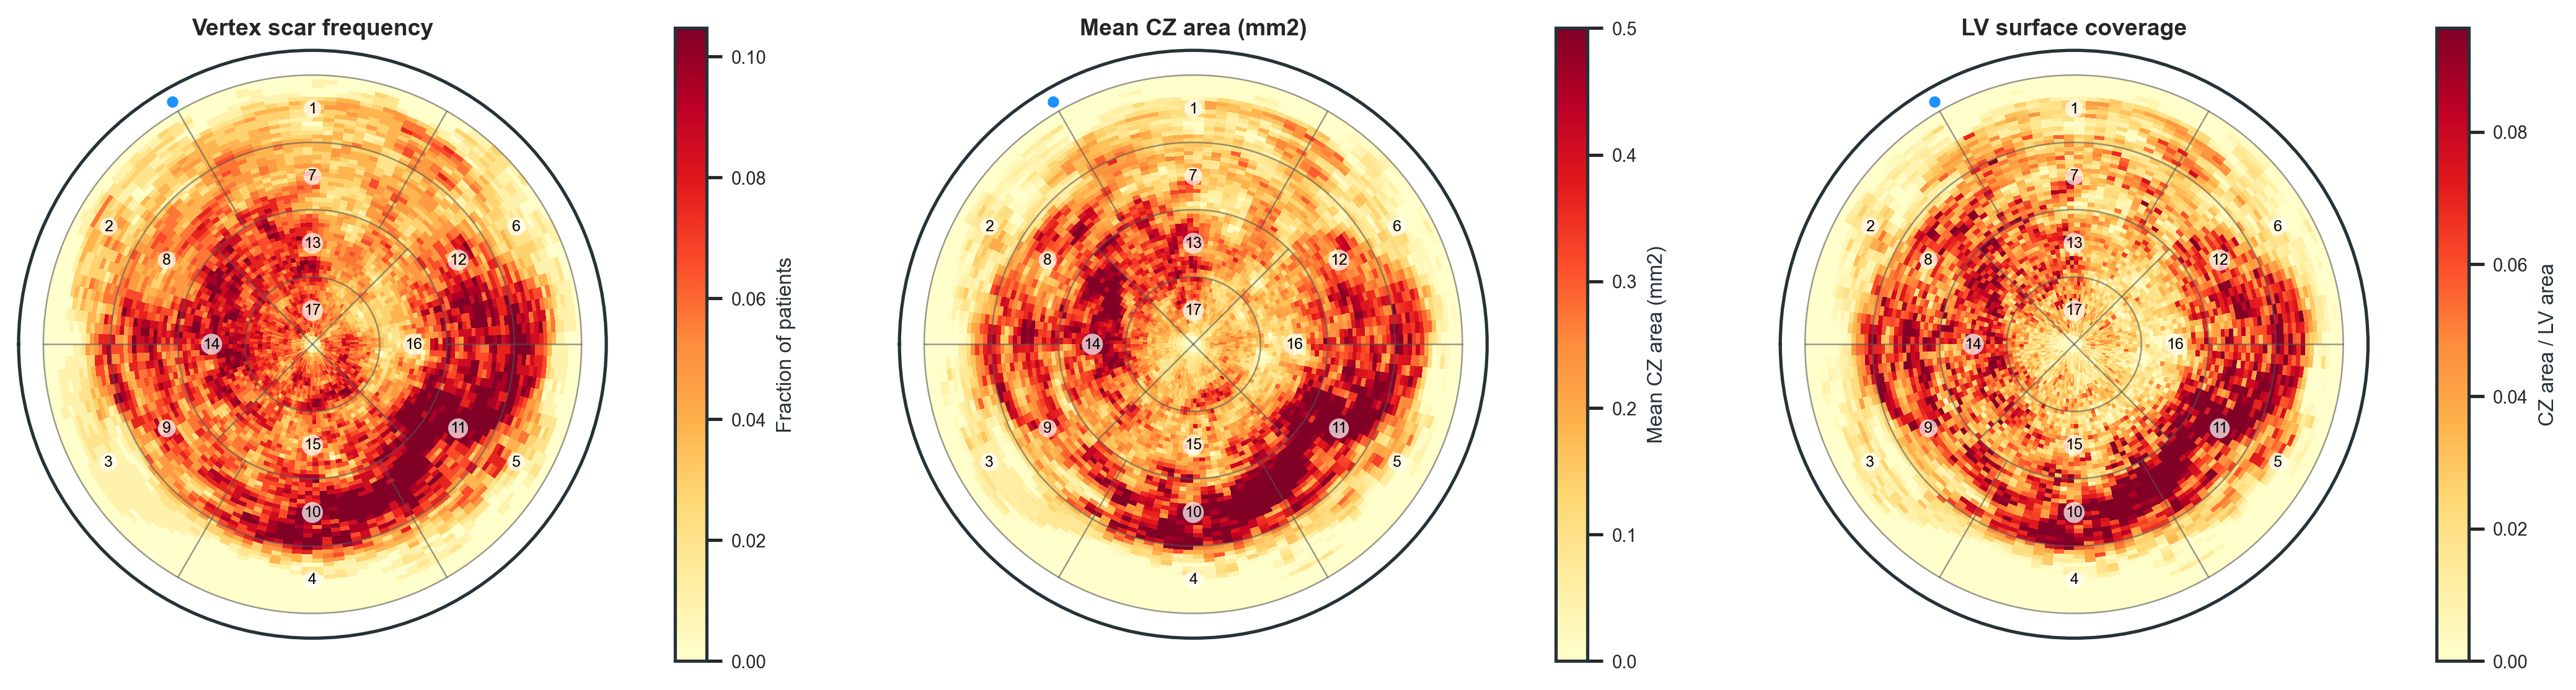
\includegraphics[width=\textwidth]{figures/fig3_population_superposition}
    \caption{Population superposition maps ($n=105$) for vertex-based, area-based, and LV coverage methods. Spatial patterns are consistent; the coverage method reveals higher RCA density obscured in vertex-based by that territory's smaller surface area.}
    \label{fig:superposition}
\end{figure}

\subsection{Grid resolution sensitivity}

The operational $64 \times 128$ polar grid was compared against a coarser ($32 \times 64$)
and a finer ($128 \times 256$) alternative. The three configurations differ substantially in
their vertex density per bin (Table~\ref{tab:grid}).

\begin{table}[htbp]
    \centering
    \caption{Grid resolution comparison.}
    \label{tab:grid}
    \begin{tabular}{lrr}
        \toprule
        Grid & Bins & Avg.\ LV vertices/bin \\
        \midrule
        $32 \times 64$ (coarse) & 2\,048 & ${\sim}24$ \\
        $64 \times 128$ (operational) & 8\,192 & ${\sim}6$ \\
        $128 \times 256$ (fine) & 32\,768 & ${\sim}1.5$ \\
        \bottomrule
    \end{tabular}
\end{table}

The $64 \times 128$ grid provides the best trade-off: ${\sim}6$ vertices per bin gives stable
binary scar detection with sufficient resolution to distinguish all 17 AHA segments. Population
mean maps are consistent across all three resolutions (Figure~\ref{fig:app_gridres} in Appendix).

\subsection{Verification of polar maps}
\label{sec:polarmapverif}

Visual inspection of representative cases shows that scar localisation is broadly consistent
between the two methods in both circumferential and longitudinal coordinates. The primary
discrepancy concerns radial density: the $r^{1/3}$ radial displacement applied by the
reference method concentrates scar representations toward the basal ring, whereas the
linear mapping used here distributes coverage more uniformly along the apex-to-base axis;
as a consequence, the proposed method recovers scar points near the apex with greater
completeness. The 3D LV reconstruction and polar map comparison for the representative case are shown in
Figure~\ref{fig:verif_combined}. More generally, the longitudinal coordinate $s$ of the
proposed method encodes apex-to-base position directly as the normalised projection onto
the long axis, providing a monotonic and geometrically interpretable representation of the
full apex-to-base gradient; the flat disk radius of the reference method is determined by the
conformal (angle-preserving) flattening transformation, whose output depends on the global
geometry of the endocardial surface and cannot be expressed as a simple function of
normalised apex-to-base position alone.
Cross-referencing with the 3D LV shell further suggests that the two methods sample
different transmural depths: the reference method labels endocardial surface points in
proximity to the Core Surface and therefore captures the endocardial face of the scar,
whereas the proposed method projects Core Surface vertices directly and therefore
represents the full transmural extent of the scar mass. Taken together, the two approaches
are complementary: differences in radial density and transmural sampling reflect distinct
mapping choices rather than errors in anatomical localisation.

\begin{figure}[ht]
    \centering
    \begin{subfigure}[b]{0.33\textwidth}
        \centering
        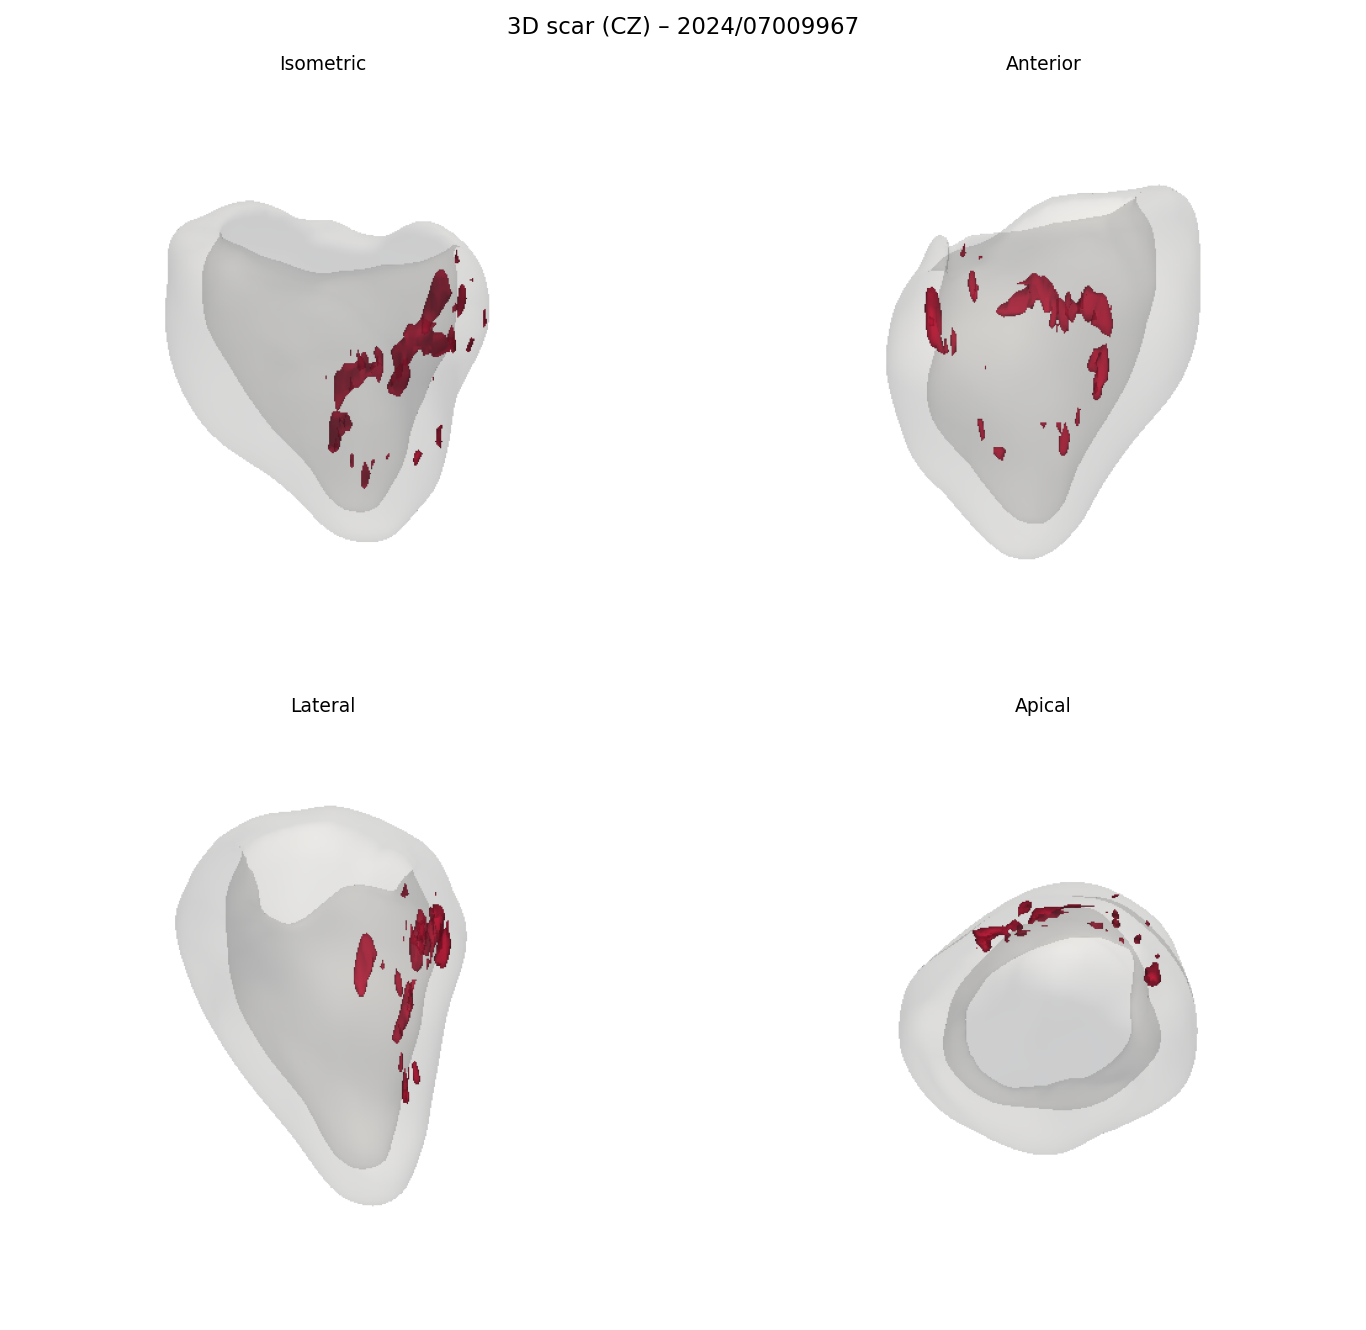
\includegraphics[width=\textwidth]{figures/M06_3d_scar_2024_07009967}
    \end{subfigure}
    \hfill
    \begin{subfigure}[b]{0.52\textwidth}
        \centering
        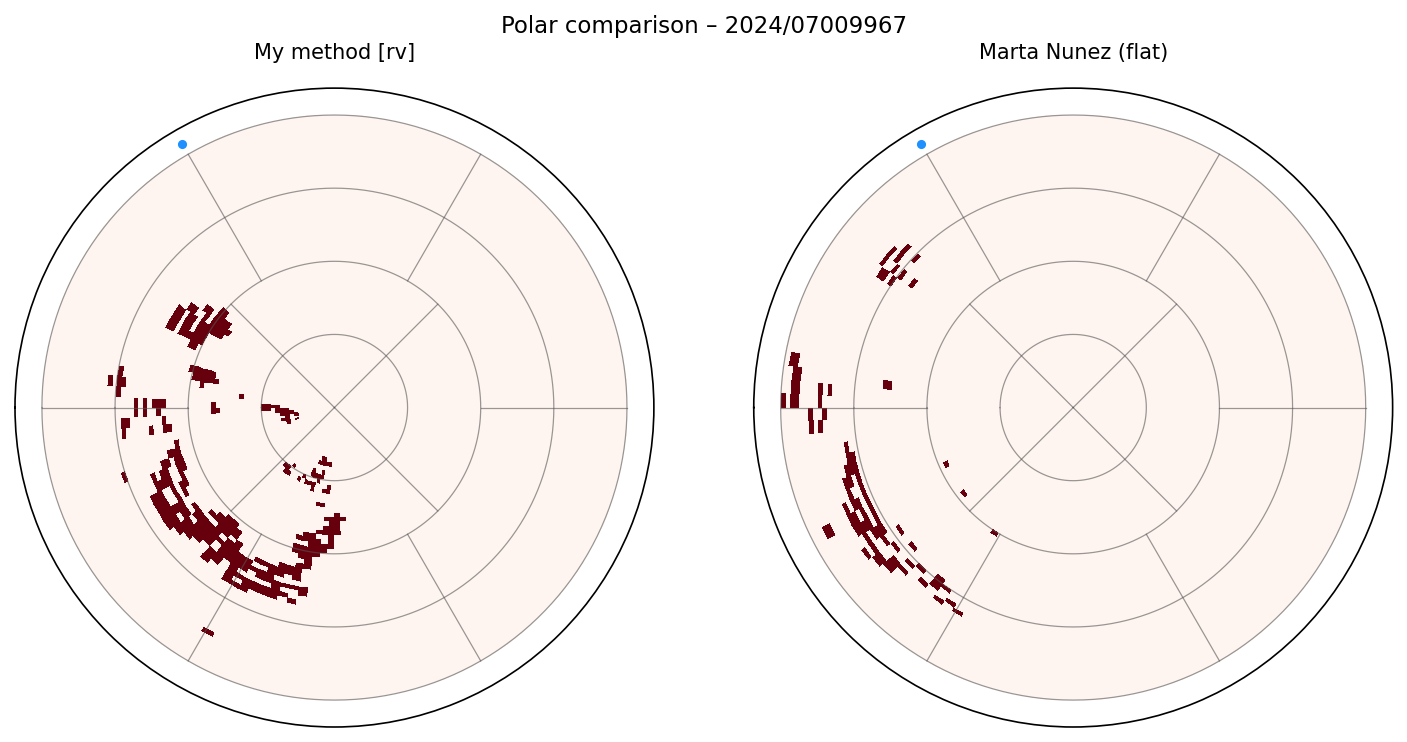
\includegraphics[width=\textwidth]{figures/M06_polar_comparison_2024_07009967}
    \end{subfigure}
    \caption{Verification for case 2024\_07009967: (a) 3D LV with core-zone scar (red); (b) polar map comparison, proposed method (left) vs.\ N\'{u}\~{n}ez Garc\'{i}a \cite{nunez2018} (right). Scar localisation is consistent; differences reflect distinct mapping choices.}
    \label{fig:verif_combined}
\end{figure}

\FloatBarrier
\section{Population-Level Scar Analysis}

All analyses used vertex-based binary polar maps on the full 105-case cohort with
non-parametric methods, as justified by the normality diagnostics below.

\subsection{Normality diagnostics}

Univariate normality was assessed via QQ plots, comparing the Pearson correlation
between sample and theoretical normal quantiles against critical values at $\alpha = 0.05$.
Only age satisfied the normality criterion. Since univariate normality is a necessary
condition for multivariate normality, the failure of all scar-related variables precludes a
multivariate normal joint distribution analytically; a chi-squared QQ plot of squared
Mahalanobis distances of the full 17-segment burden vector was computed to corroborate
this visually.

All scar-related variables showed strong zero-inflation and right skewness: at the AHA
segment level, 70--75\% of patients had zero scar in most segments, with mean/median
ratios of 2.4--3.7 and SD/mean ratios of 2--4. Territory-level and global burden variables
showed similar patterns, with less extreme zero-inflation due to bin aggregation. All
subsequent analyses therefore used non-parametric methods (Friedman test, Wilcoxon
signed-rank, Spearman rank correlation) and patient-level bootstrap confidence intervals
(2\,000 resamples).

\subsection{AHA-17 segment burden and population atlas}

A notable structural property of the segment-level distributions is the dissociation between
prevalence and extent: a segment can be frequently affected yet carry low mean burden, or
rarely affected but carrying high conditional burden when it is. This arises directly from
zero-inflation---the unconditional mean is dragged toward zero even when the conditional
mean among affected patients is substantial. Segment-level summaries therefore report both
quantities separately. For example, the basal inferolateral segment (seg 5) is scar-positive
in 44.8\% of patients yet carries an unconditional mean burden of only 0.032, because the
majority of patients contribute a zero; the apical septal segment (seg 14) is affected in a
similar proportion of patients (41.0\%) but, when involved, carries a conditional mean burden
of 0.190---nearly six times higher.

The Friedman test confirmed that scar burden is non-uniformly distributed across the 17 AHA
segments within patients ($p = 3.3 \times 10^{-17}$, $n = 105$). Although
this result is anatomically expected---ischaemic infarction follows coronary territory
boundaries, making uniform distribution implausible a priori---the formal test establishes that
the data are internally consistent with anatomical priors. Post-hoc pairwise Wilcoxon signed-rank tests with
Bonferroni correction (136 comparisons, adjusted threshold $\alpha = 0.000368$) identified
20 segment pairs with statistically significant burden differences. The significant pairs were
not distributed uniformly across the LV: they were concentrated between the inferior and
inferoseptal mid-ventricular segments (segments 9--11) and the anterior basal segments
(segments 1--4), with mid inferior (segment 10) and mid inferolateral (segment 11) emerging
as the segments most consistently distinguishable from the rest of the wall. No significant
differences were found among segments within the same anatomical ring (i.e.\ segments
sharing the same apex-to-base level, such as the six basal segments 1--6) or between
neighbouring segments in the lateral basal region, where scar burden values were similarly
low across adjacent sectors, indicating that the spatial heterogeneity is structured rather
than diffuse: the significant pairwise differences are not scattered randomly across the 136
comparisons but concentrate specifically between the inferior mid-ventricular segments
(10--11, highest burden) and the anterior basal segments (1--4, lowest burden), a pattern
consistent with the anatomical boundaries of the RCA and LAD territories.

Bootstrap confidence intervals confirm a statistically robust spatial hierarchy. Basal
segments (1--4, mean 0.014--0.023) are clearly and reliably spared: their CI upper bounds
($\leq 0.035$) do not overlap with the CI lower bounds of the mid-cavity hotspot segments
(segs 10--11, CI lower $\geq 0.061$). The mid-inferolateral segment (seg 11, mean = 0.100,
95\% CI [0.070, 0.135]) is the single most affected region, followed by the mid-inferior
(seg 10, mean = 0.088) and apical septal (seg 14, mean = 0.078) segments. The wide CIs
of hotspot segments reflect the high inter-patient variability driven by zero-inflated,
right-skewed distributions. The population atlas identifies a robust inferior-to-apical hotspot
centred on the mid-inferolateral and mid-inferior segments (AHA 11 and 10), straddling the
RCA--LCX boundary, with basal segments consistently spared.

% [FIGURE PLACEHOLDER --- archetype/atlas map to be inserted]
The bootstrap population mean polar map is provided in Appendix~\ref{app:atlas}.

\subsection{Coronary territory burden and archetype maps}
\label{sec:terrburden}

The 2\% threshold for territory involvement was selected via sensitivity analysis across
candidate values (1\%, 2\%, 3\%, 5\%, 10\%); the full sensitivity curve is shown in
Figure~\ref{fig:app_territory_threshold} in the Appendix. At 1\% the multi-territory fraction
exceeded 60\%, implausibly high for a focal-infarct cohort; thresholds above 3\%
progressively assigned no-scar classification to patients with minor genuine involvement.
The 2\% value represents the earliest stable point at which single-territory classification
reaches its plateau and the no-scar fraction remains low (${\sim}10\%$).

LCX showed the numerically highest mean territory burden (0.055), followed by LAD (0.051)
and RCA (0.047). These differences were not statistically significant ($p = 0.148$), indicating no systematic coronary territory preference at the
population level. Ring-level analysis showed that the apical and mid-cavity rings carry the
highest scar involvement, with the basal ring consistently spared.

Archetype maps stratified by dominant territory reveal distinct spatial geometries. LAD-dominant
scar is the most diffuse: it extends longitudinally from the anteroseptal segments down through
the apex (segment 17), producing an elongated pattern along the long axis that spans multiple
rings. RCA- and LCX-dominant scar, by contrast, tends toward circumferential spread at the
mid-cavity level, wrapping around the inferior and lateral walls with less longitudinal extension.
This difference reflects the anatomical territory boundaries: the LAD supplies the anterior wall
and apex, while RCA and LCX supply the inferior and lateral walls, which are arranged more
circumferentially in the mid-ventricular ring.

The lower vertex-based RCA burden does not imply geometrically insignificant infarction:
as shown by the coverage analysis (Section~\ref{sec:projmethods}), RCA scar tends to be
locally concentrated when present: the total scar surface area per bin classified as
scar-positive is higher for RCA than for LCX or LAD, meaning RCA scar packs more tissue
area into a smaller number of bins.

The area-based and vertex-based analyses produced concordant spatial rankings at both
segment and territory levels (Spearman $\rho > 0.85$ across all 17 segments and all three
territories), and both Friedman tests reached the same inferential conclusions, supporting
consistency across methodologically independent quantification approaches.

\subsection{Inter-segment correlation structure and PCA}

The $17 \times 17$ Spearman inter-segment correlation matrix reveals a block-diagonal
structure aligned with coronary territories: segments within the same territory co-vary
positively, consistent with shared vascular supply causing contiguous infarction. Importantly,
the dominant within-territory correlation pattern is longitudinal (apex-to-base) rather than
circumferential---vertically adjacent segments (e.g.\ seg 5 and seg 11, both LCX but at
different ring levels) show higher correlations than circumferentially adjacent segments in
different territories, indicating that scar penetrates transmurally along the wall depth rather
than spreading circumferentially. Inter-territory correlations are weak, with the smallest
observed between LCX and RCA ($\rho = 0.114$), supporting the treatment of territory
burdens as approximately independent dimensions.

PCA of the $z$-score standardised 17-segment vectors shows that six components are
needed to explain 72\% of the variance, with PC1 accounting for only 18\%. This low
concentration of variance in the first component indicates that no single spatial mode
dominates scar variability---the scar pattern space is intrinsically high-dimensional, reflecting
the diversity of infarct locations and extents across the cohort.

\subsection{Age and sex associations}

No segment reached significance after Bonferroni correction ($\alpha = 0.05/17$, $n = 48$).
Numerically strongest trends: mid-inferior seg~10 ($\rho = 0.345$, $p_\text{Bonf} = 0.280$)
and apex seg~17 ($\rho = -0.307$, $p_\text{Bonf} = 0.575$); RCA territory $\rho = 0.285$
($p = 0.050$, n.s.). Sex-stratified analysis was not performed due to severe imbalance
(38 male / 10 female).

\subsection{Transmurality}

Figure~\ref{fig:transmurality_combined} shows
fragment-level onset and transmurality stratified by ring zone and coronary territory. Onset measures the shallowest wall depth at which scar begins (0 =
endocardial, 1 = epicardial); transmurality is the span from onset to outermost depth. Both
are derived from the continuous vertex-depth computation described in
Section~\ref{sec:statistical}.

The continuous vertex-depth approach yields a mean fragment onset of 0.300 and a mean
fragment transmurality of 0.190, indicating that scar originates near the endocardial surface
and extends approximately 19\% of wall thickness---consistent with subendocardial ischaemic
infarction. Onset is lowest in the apical and mid rings and highest in the basal ring.
This is expected because coronary occlusions most commonly occur at mid-artery levels;
the ischaemic wavefront propagates from the occluded segment outward, reaching basal
myocardium last and with reduced severity, so scar there tends to begin deeper in the wall.
By coronary territory, RCA presents the highest onset (mean 0.318) and the highest
transmurality (mean 0.216), making it the most deeply penetrating territory in this cohort.

The transmurality gradient analysis shows a positive population-mean core-to-edge
difference, confirming a dense-core / thin-edge transmural structure: the central scar mass
extends more deeply through the wall than its periphery.

Endocardial dominance was confirmed at the cohort level: on average 65\% of scar-positive
bins per patient showed onset $\leq 30\%$ of wall thickness (endocardial), 20\% fell in the
midwall range (30--60\%), and 15\% showed epicardial-dominant onset ($> 60\%$).

\begin{figure}[htbp]
    \centering
    \begin{subfigure}[t]{0.48\textwidth}
        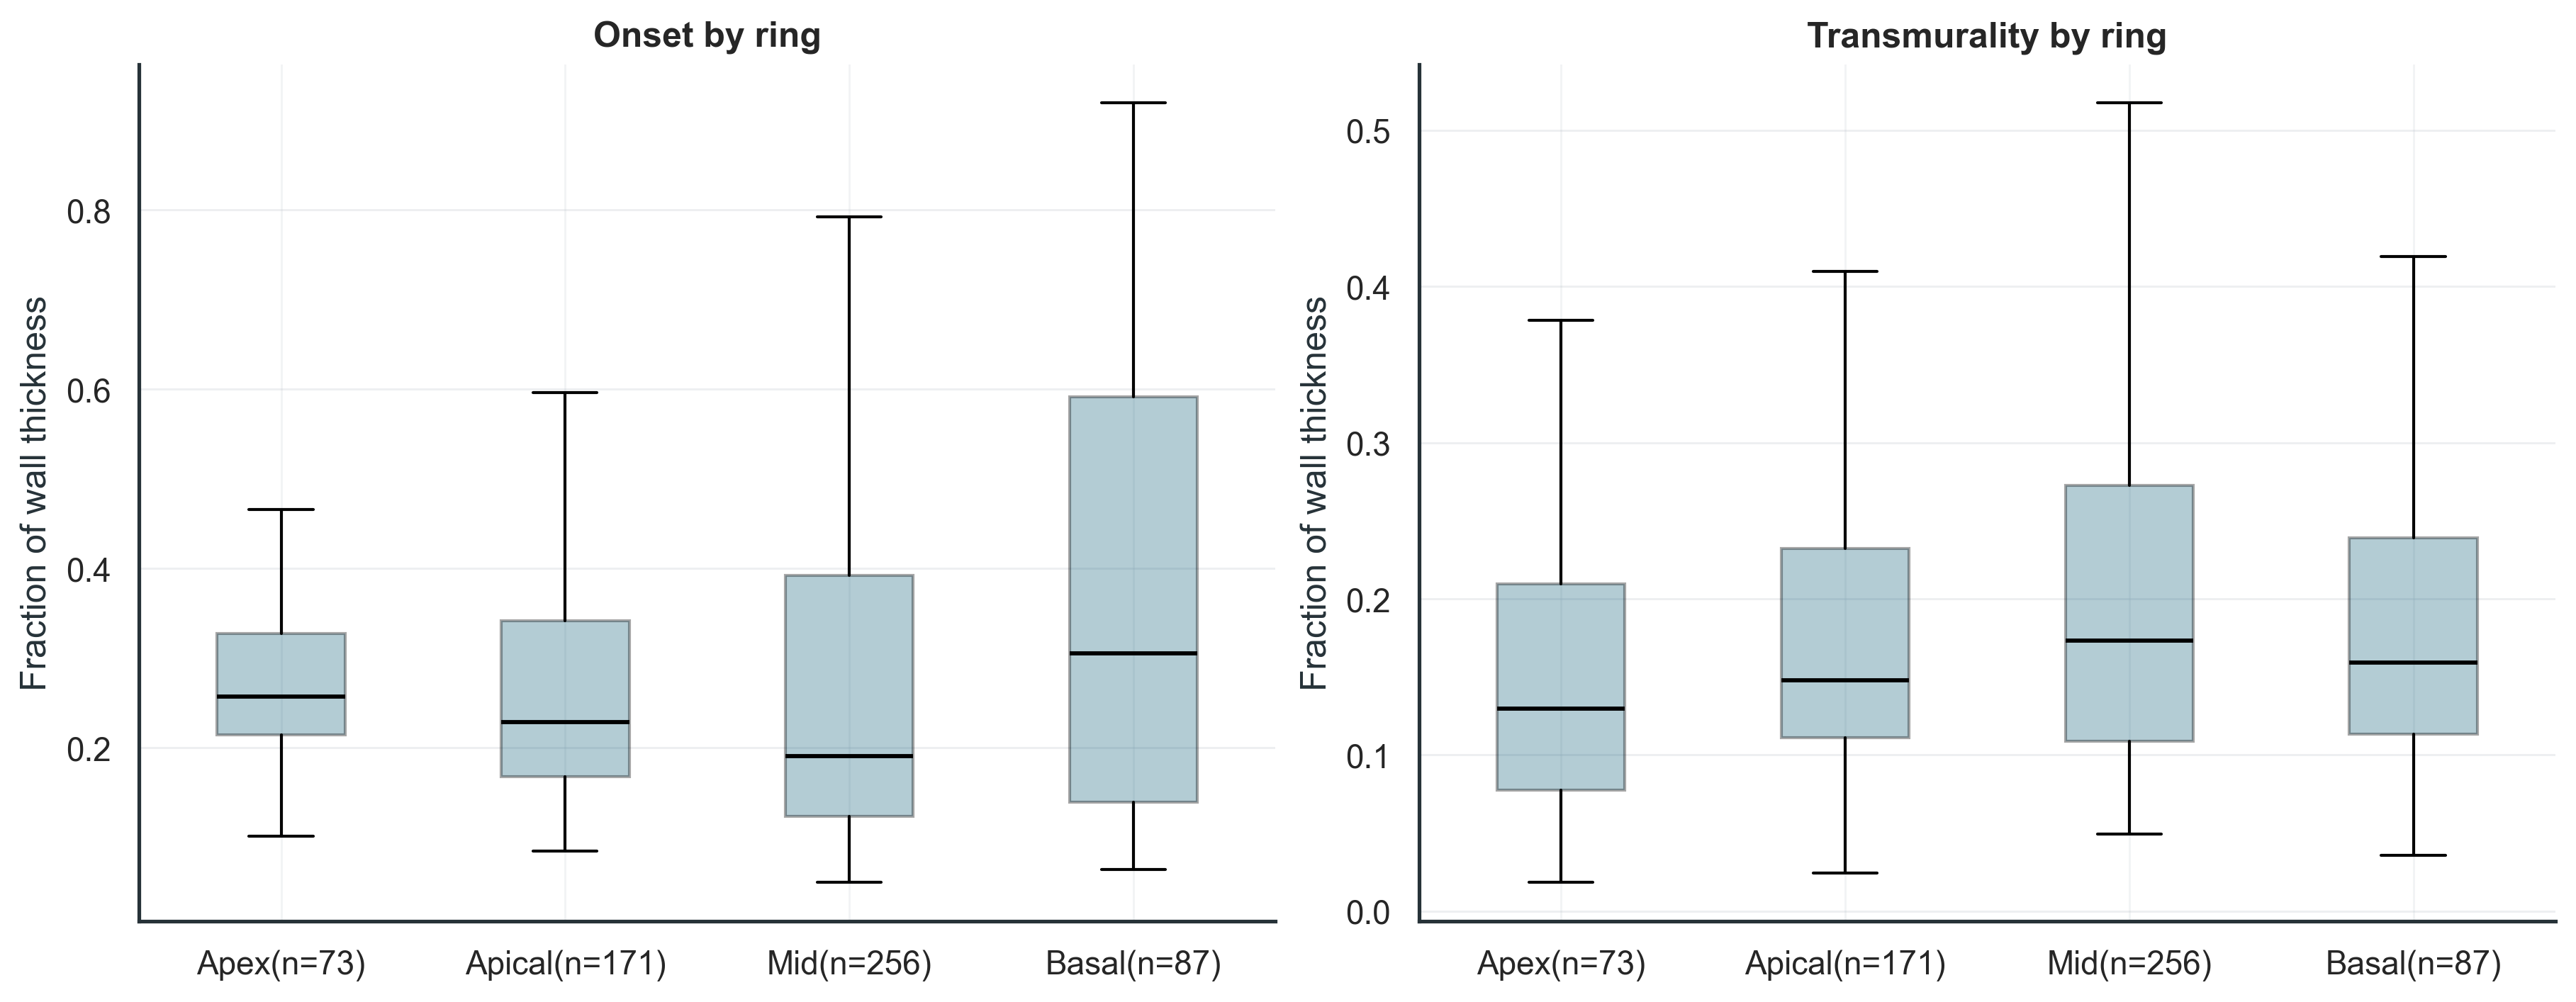
\includegraphics[width=\textwidth]{figures/fragment_onset_transmurality_by_ring}
    \end{subfigure}
    \hfill
    \begin{subfigure}[t]{0.48\textwidth}
        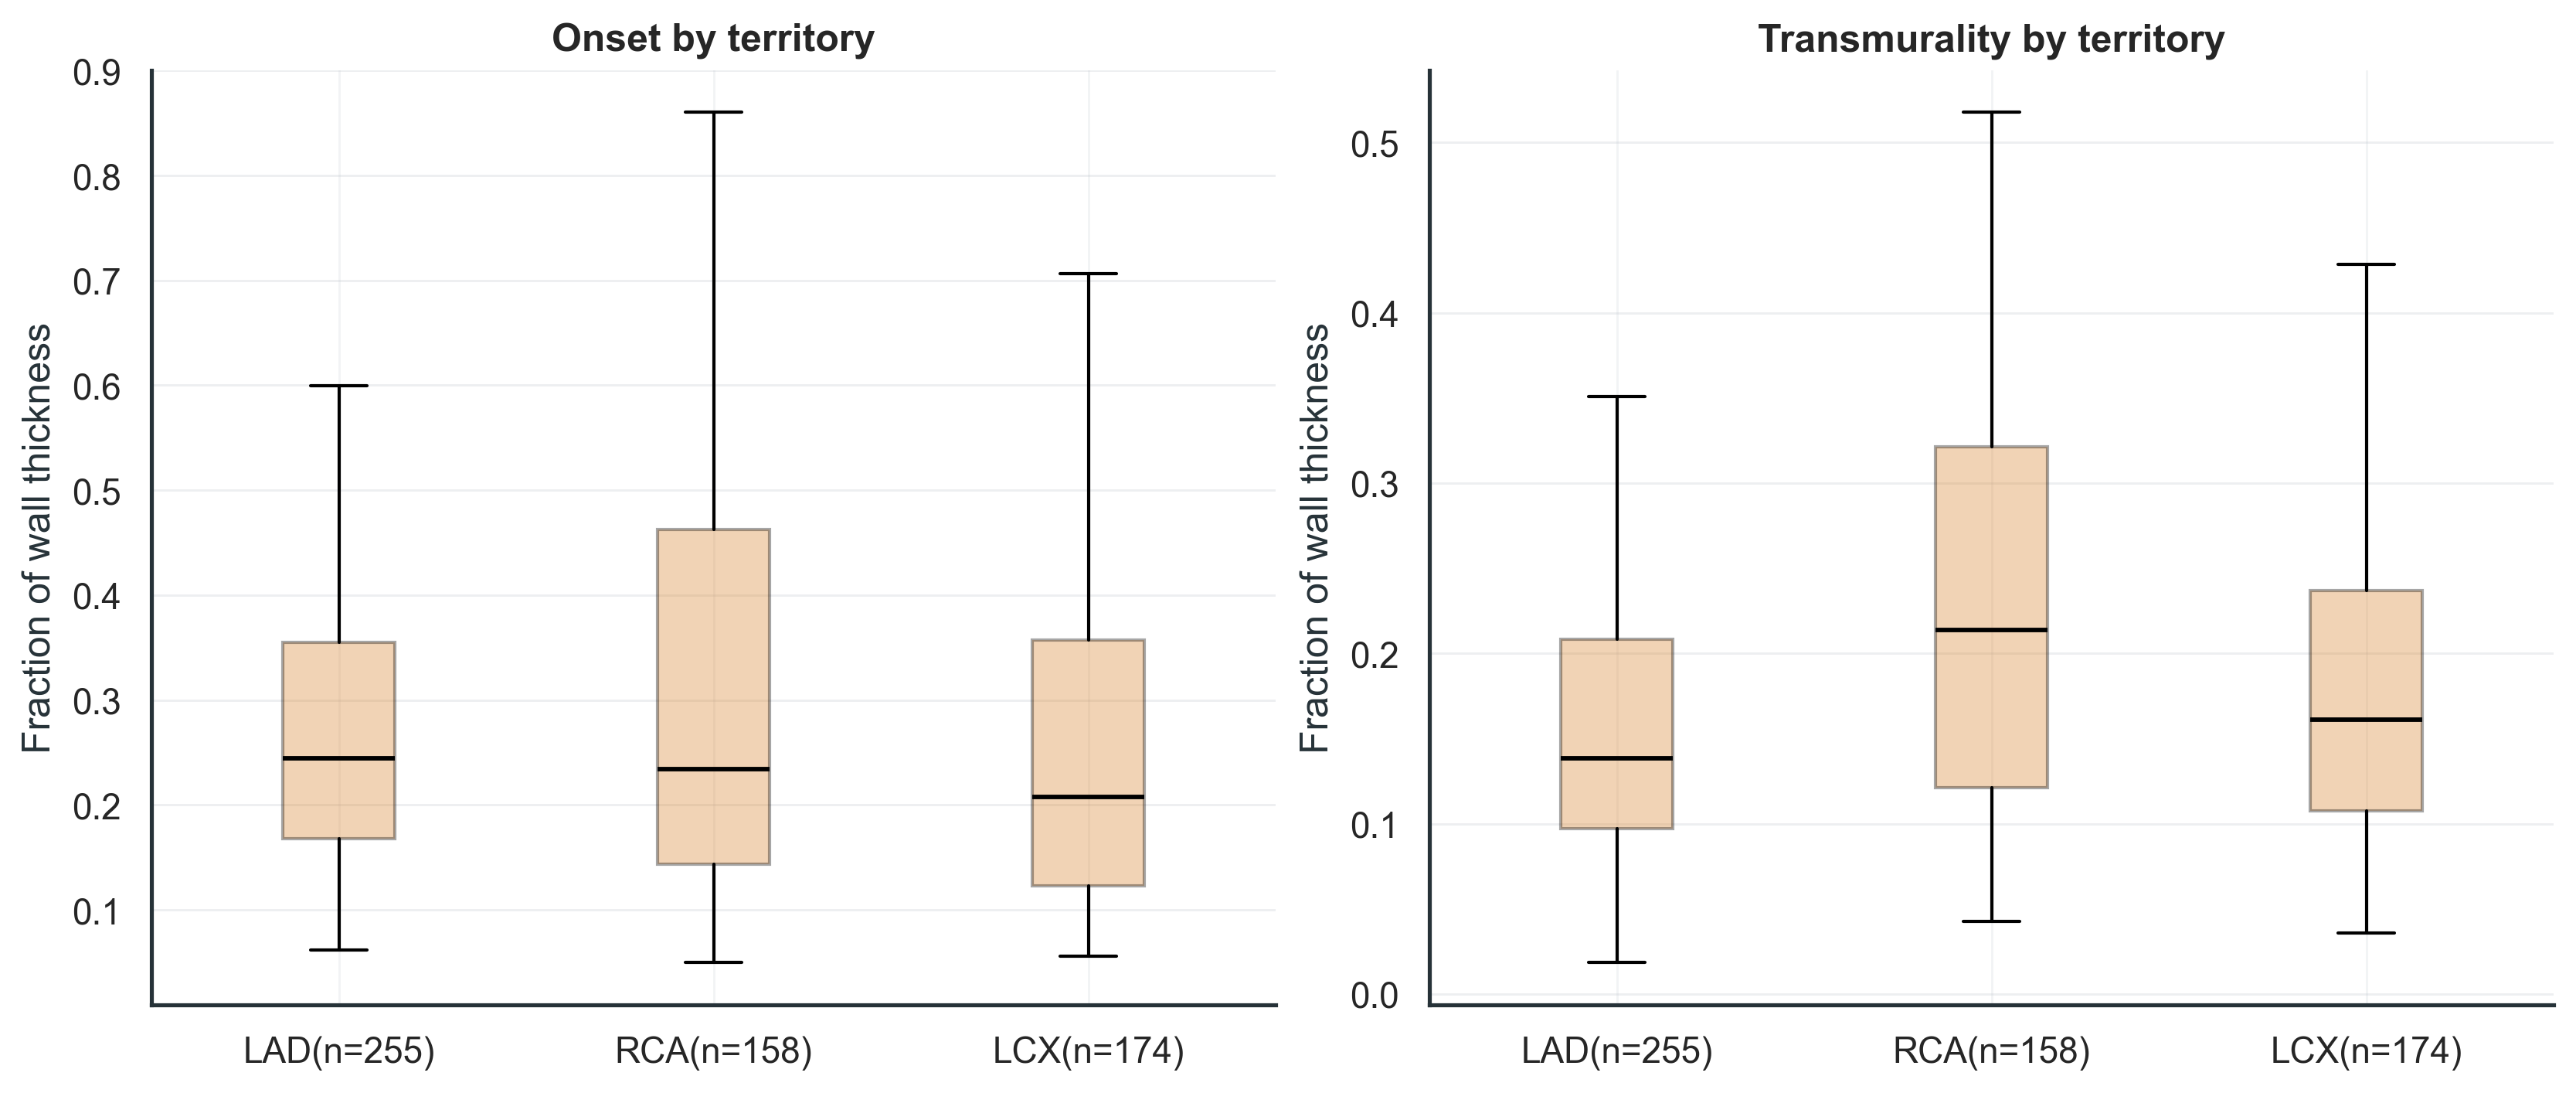
\includegraphics[width=\textwidth]{figures/fragment_onset_transmurality_by_territory}
    \end{subfigure}
    \caption{Fragment-level onset and transmurality stratified by (a) ring zone and (b) coronary territory.
    Onset = shallowest wall depth at which scar begins (0 = endocardial, 1 = epicardial);
    transmurality = span from onset to outermost depth, both derived from the continuous
    vertex-depth method (Section~\ref{sec:statistical}).}
    \label{fig:transmurality_combined}
\end{figure}

\vspace{-0.8em}
\subsection{Geometric descriptors and fragment shape}

Within-patient Spearman correlation between the 17-element segment-level extent vector
and the 17-element per-segment mean transmurality vector yielded a median $\rho = 0.571$
(mean 0.547, IQR [0.359, 0.800]; $n = 97$ patients with computable correlation, i.e.\ at
least three AHA segments with both valid transmurality and positive scar extent; the
remaining 8 patients had insufficient scar-positive segments for a valid rank correlation),
confirming partial but incomplete association: in most patients more-burdened segments
tend to penetrate more deeply, but the relationship is far from deterministic.

The apex-to-base scar gradient showed near-zero population means (linear slope:
$-0.031 \pm 0.165$; Spearman $\rho$: $+0.088 \pm 0.425$) with extreme inter-patient
variability: slopes ranged from $-0.82$ (strongly apex-dominant) to $+0.20$ (base-dominant),
and $\rho$ from $-0.89$ to $+0.74$. When averaged across the cohort, no dominant
longitudinal preference is detected by the apex-to-base gradient analysis; however, at the
individual level the gradient discriminates strongly between apex-dominant and base-dominant
patterns, and other analyses---notably the territory archetype maps---do reveal longitudinal
differences once patients are stratified by coronary territory.

Shape analysis of the largest scar fragment showed that most patients present irregular,
non-compact lesions (median compactness 0.39). The mid ring is where scar appears most
circumferentially spread.

\FloatBarrier
\section{Retrieval-Based Scar Generation}

This section reports the leave-one-out retrieval evaluation: feature vector comparison,
distance metric selection, and performance statistics under deterministic and probabilistic
modes.

\subsection{Feature vector comparison and selection}

Six candidate descriptor vectors were evaluated under leave-one-out retrieval with Manhattan
distance. Table~\ref{tab:featurevectors} and Figure~\ref{fig:featurevectors} report their
dimensionality and the three retrieval quality metrics. SVD scree plots and patient PC1--PC2
scatter plots for all vectors are provided in Figure~\ref{fig:app_svd_plots} in the Appendix.

\begin{table}[htbp]
    \centering
    \caption{Leave-one-out (LOO) retrieval performance, six descriptor vectors (Manhattan distance, $n=105$). Mean and median $|\Delta\text{CZ}|$ lower is better; Seg/Polar Dice higher is better.}
    \label{tab:featurevectors}
    \small
    \begin{tabular}{lrrrrrr}
        \toprule
        Vector & Feats & Mean $|\Delta\text{CZ}|$ & Med $|\Delta\text{CZ}|$ & Seg Dice & Polar Dice \\
        \midrule
        \textbf{full}        & \textbf{39} & 0.0148 & 0.0093 & \textbf{0.597} & 0.106 \\
        full\_no\_seg        & 22 & \textbf{0.0130} & \textbf{0.0079} & 0.489 & 0.100 \\
        full\_pruned         & 29 & 0.0188 & 0.0105 & 0.545 & 0.109 \\
        full\_ns\_pruned     & 16 & 0.0189 & 0.0115 & 0.474 & 0.093 \\
        pmap\_only           &  8 & 0.0188 & 0.0087 & 0.359 & \textbf{0.214} \\
        full\_ns+pmap        & 30 & 0.0136 & 0.0076 & 0.484 & 0.155 \\
        \bottomrule
    \end{tabular}
\end{table}

\begin{figure}[tb]
    \centering
    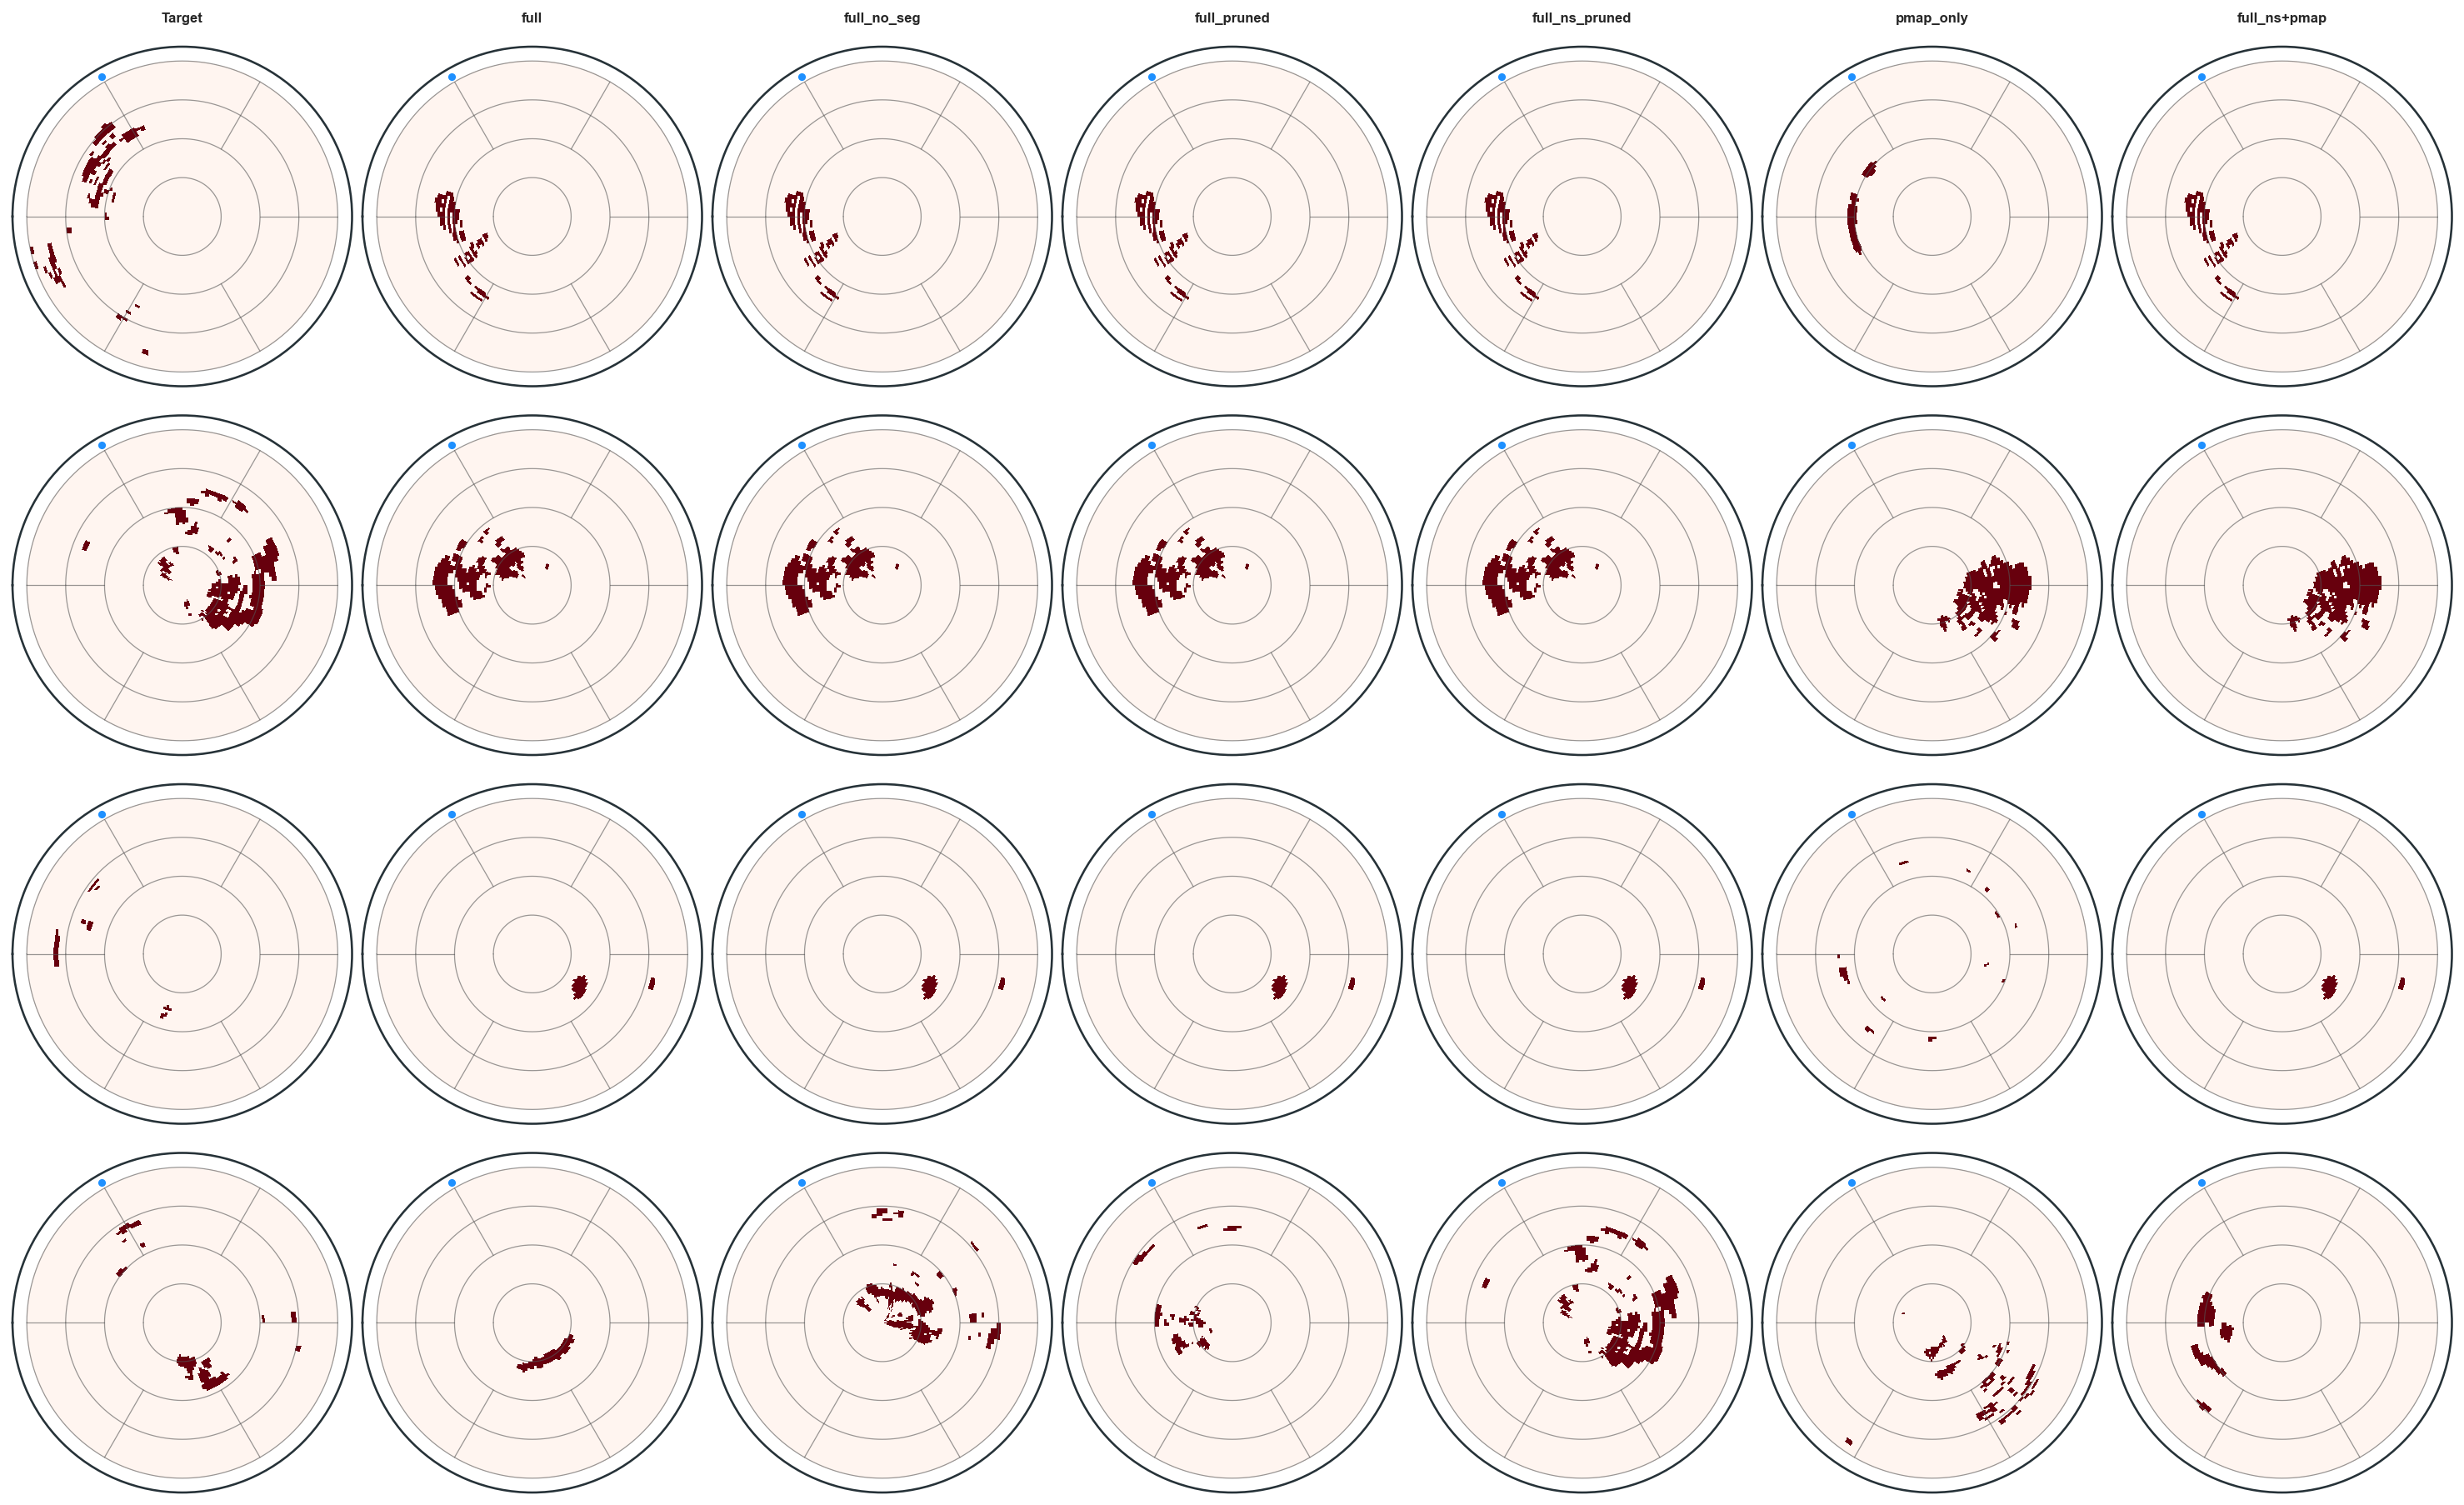
\includegraphics[width=0.80\textwidth]{figures/retrieval_six_vectors}
    \caption{Leave-one-out (LOO) retrieval performance for seven descriptor vectors
    (Manhattan distance, $n=105$). Columns from left to right: (1) target patient;
    (2)~\texttt{full} (39 features, all structured descriptors including AHA segment burdens);
    (3)~\texttt{full\_no\_seg} (22 features, structured descriptors without per-segment burdens);
    (4)~\texttt{full\_pruned} (29 features, \texttt{full} after SVD-based pruning);
    (5)~\texttt{full\_ns\_pruned} (16 features, \texttt{full\_no\_seg} after pruning);
    (6)~\texttt{pmap\_only} (8 features, principal component analysis (PCA) scores of binary polar maps);
    (7)~\texttt{full\_ns+pmap} (30 features, non-segment structured descriptors combined with polar-map PCA scores).}
    \label{fig:featurevectors}
\end{figure}

SVD analysis showed AHA segment features dominate variance (16 vs.\ 11 components for
90\% coverage in the segment-free variant). Feature pruning degraded performance on two
of three metrics (burden error 0.015$\to$0.019; segment Dice 0.597$\to$0.545), indicating
discriminative information is distributed across low-variance dimensions.
\textbf{pmap\_only} achieved highest polar-map Dice (0.214) but lowest segment Dice (0.359)
and worst burden error. The full 39-feature vector achieved the best segment-level Dice and
was selected as the primary descriptor because segment-level anatomical overlap was
prioritised and the features remain interpretable. However, it did not achieve the best value
on every metric: \textbf{full\_no\_seg} had the lowest scar burden error (0.0130
vs.\ 0.0148), and \textbf{pmap\_only} achieved the highest polar-map Dice (0.214
vs.\ 0.106). This shows that descriptor choice depends on the intended retrieval target.

\vspace{-0.8em}
\subsection{Distance metric comparison}

Manhattan distance on $z$-score normalised features outperformed Euclidean (segment Dice
0.597 vs.\ 0.539) and substantially outperformed cosine (segment Dice 0.282), which is
insensitive to vector magnitude.

\subsection{Performance on Territories and Deterministic and Probabilistic Retrieval}

Retrieval performance varied systematically by dominant coronary territory
(Table~\ref{tab:terrperf}): LCX-dominant patients achieved the lowest burden error
(mean $|\Delta\text{CZ}| = 0.010$) and highest segment Dice (0.629), followed by RCA
(0.013, 0.612) and LAD (0.023, 0.518). LAD-dominant scar---which extends longitudinally
across multiple rings---is harder to match than the more circumferentially localised RCA
and LCX patterns.

\begin{table}[htbp]
    \centering
    \caption{Leave-one-out (LOO) retrieval performance by dominant coronary territory and number of involved
    territories (full vector, Manhattan distance, $n=105$). $|\Delta\text{CZ}|$ = absolute core-zone (CZ) burden error;
    Seg Dice = segment-level Dice overlap over the AHA 17-segment model;
    Polar Dice = pixel-level overlap on the $64\times128$ polar grid.}
    \label{tab:terrperf}
    \small
    \begin{tabular}{lrrrr}
        \toprule
        Group & $n$ & Mean $|\Delta\text{CZ}|$ & Seg Dice & Polar Dice \\
        \midrule
        \multicolumn{5}{l}{\textit{By dominant territory}} \\
        LAD (Anterior) & 33 & 0.023 & 0.518 & 0.171 \\
        RCA (Inferior) & 31 & 0.013 & 0.612 & 0.064 \\
        LCX (Lateral)  & 41 & 0.010 & 0.629 & 0.086 \\
        \midrule
        \multicolumn{5}{l}{\textit{By number of involved territories}} \\
        1 territory & 40 & 0.012 & 0.550 & 0.090 \\
        2 territories & 41 & 0.015 & 0.533 & 0.141 \\
        3 territories & 13 & 0.034 & 0.617 & 0.122 \\
        \bottomrule
    \end{tabular}
\end{table}

By number of involved territories, single-territory patients showed the lowest burden error
(0.012), consistent with better case-base coverage of focal patterns. Three-territory patients
showed the highest burden error (0.034), reflecting that diffuse multi-territory scar is rare
enough to lack close matches among the remaining 104 cases.

In practice, the softmax weights are strongly concentrated on the nearest neighbour when its
distance is substantially smaller than the second-nearest. This was observed for several
patients in the cohort, where the nearest neighbour received sampling probability close to
1.0, making the probabilistic and deterministic modes effectively equivalent for those cases.
For patients whose top-10 neighbours are more evenly spaced in descriptor space, the
probabilistic mode distributes weight across multiple candidates, allowing different plausible
scar patterns to be returned for the same query.

A quantitative comparison across all 105 patients showed that the deterministic mode
achieves marginally better mean retrieval quality on all three metrics ($|\Delta\text{CZ}| =
0.015$, segment Dice $= 0.597$, polar-map Dice $= 0.106$) compared to probabilistic
sampling ($|\Delta\text{CZ}| = 0.016$, segment Dice $= 0.570$, polar-map Dice $= 0.104$).
The small performance gap confirms that the deterministic nearest neighbour remains the
best single match, while the probabilistic mode provides a mechanism for generating a
distribution of plausible alternatives reflecting genuine population-level variability among
patients with similar scar profiles.

\subsection{Leave-one-out validation: population-level statistics}

The full leave-one-out evaluation was performed across all 105 patients using the full vector
and Manhattan distance. Full summary statistics are reported in Table~\ref{tab:loostats} in
the Appendix; metric distributions are shown in Figure~\ref{fig:loostats}.

The $|\Delta\text{CZ}|$ distribution is right-skewed (mean 0.015, SD 0.019, median 0.009):
most retrievals show small burden discrepancies, but the right tail (up to 0.106) corresponds
to patients at the extremes of the scar burden distribution where few similar cases remain.
Segment Dice (mean 0.597, median 0.667, IQR [0.500, 0.800]) confirms that on average
two thirds of the target's involved segments are correctly identified; cases with low overlap
tend to correspond to multi-territory or diffuse patterns underrepresented in the cohort.
Polar-map Dice (mean 0.106, median 0.032) is lower by construction---two patients can
share the same involved segments while differing in sub-segment location and local
extent---but the right tail (75th percentile 0.189, max 0.529) quantifies the subset of
patients for whom a geometrically close match exists.

\begin{figure}[ht]
    \centering
    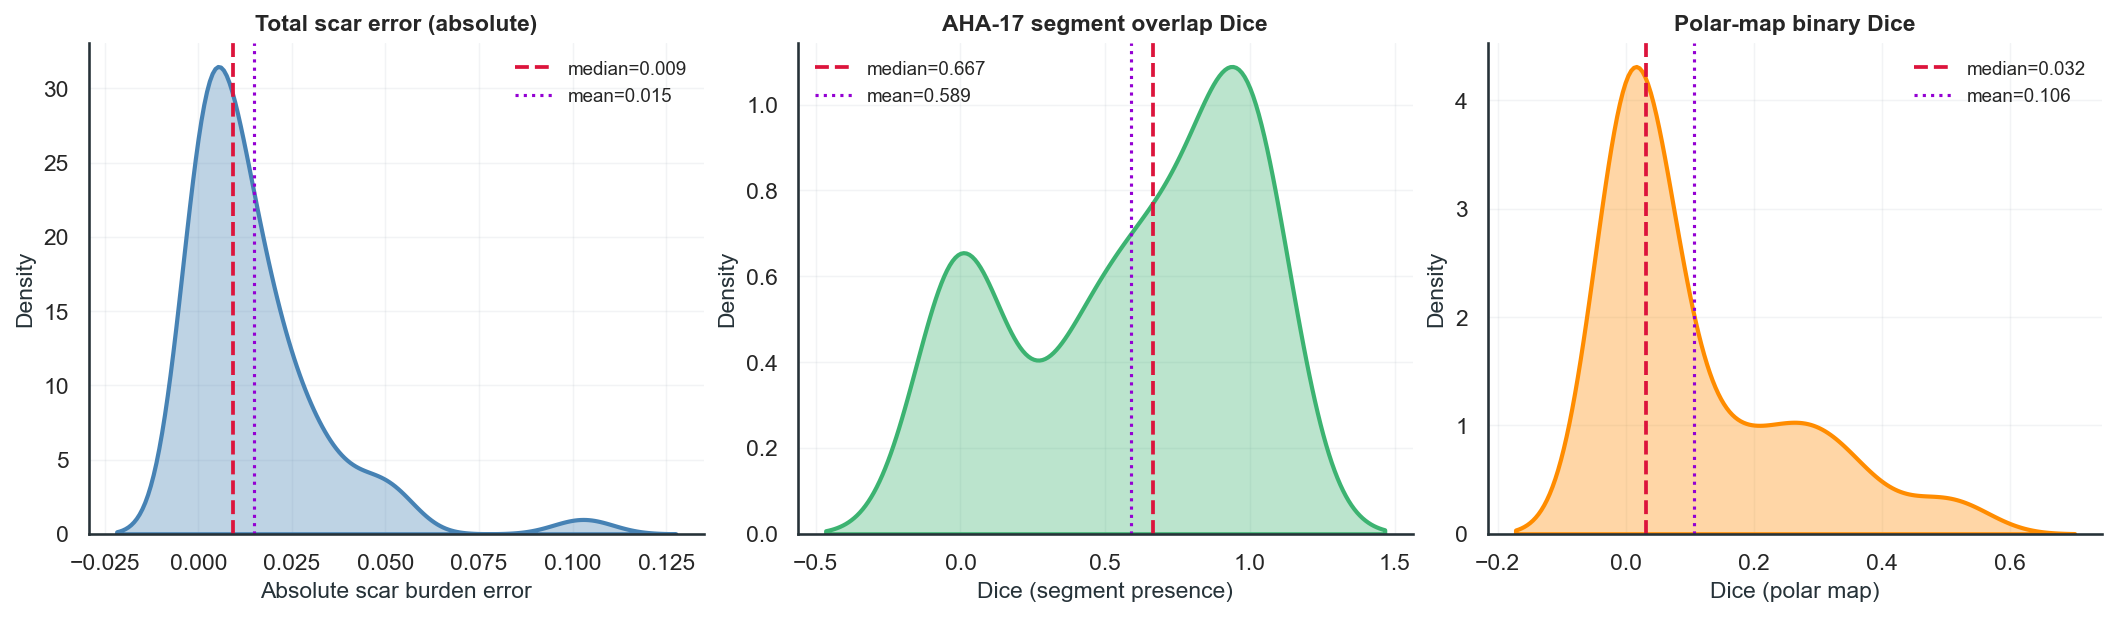
\includegraphics[width=0.70\textwidth]{figures/loo_error_distributions}
    \caption{LOO metric distributions ($n=105$, full vector, Manhattan). Top: $|\Delta\text{CZ}|$ (mean 0.015, median 0.009). Middle: segment Dice (mean 0.597, median 0.667). Bottom: polar-map Dice (mean 0.106, median 0.032).}
    \label{fig:loostats}
\end{figure}


\chapter{Discussion}

\section{Spatial Non-Uniformity and Its Anatomical Interpretation}

The statistically confirmed non-uniform distribution of scar burden across the AHA segments
is anatomically expected: ischaemic infarction follows coronary territory boundaries, making
a spatially uniform distribution implausible a priori. The value of the formal test is therefore
not surprise but documentation---it establishes that the data are internally consistent with
anatomical priors and provides a quantitative benchmark against which any generative
model must be evaluated. The concentration of burden in the inferior-to-apical
mid-ventricular wall, straddling the RCA--LCX boundary, aligns with the known vulnerability
of this region to multi-territory watershed ischaemia and with electrophysiological mapping
studies that consistently identify the inferoseptal and inferolateral walls as common sites for
re-entrant VT circuits \cite{mahida2017}. The reliable sparing of the basal ring reflects the
lower probability of occlusion at the proximal segments of all three coronary
territories---basal involvement requires either a proximal occlusion or extensive downstream
wavefront propagation, both anatomically less frequent than mid-artery occlusion.

The absence of a significant territory-level burden difference should not be read as evidence
that culprit vessel is geometrically irrelevant. The territory archetype maps demonstrate that
LAD-, RCA-, and LCX-dominant scars occupy distinct spatial footprints that scalar mean
burden cannot distinguish. This dissociation between scalar and geometric information is
precisely the limitation of existing risk stratification approaches highlighted in the
introduction: global metrics such as total scar burden or ejection fraction compress spatial
structure that is mechanistically relevant to arrhythmogenesis \cite{mahida2017}. The
present characterization, by preserving spatial information in the polar-map representation,
is positioned to contribute features that scalar approaches discard.

The high dimensionality of the scar pattern space---six PCA components for 72\% of
variance, PC1 accounting for only 18\%---has a direct mechanistic interpretation: infarct
location, extent, transmurality, and longitudinal distribution vary largely independently across
patients, producing a genuinely high-dimensional population distribution. This stands in
contrast to healthy cardiac anatomy, where statistical shape models typically achieve
compact low-dimensional representations because morphological variability is constrained
by developmental and functional pressures \cite{rodero2021, doste2026}. Post-infarction scar
geometry is not so constrained: the location and extent of ischaemic injury depend on which
vessel occludes, at what level, and for how long---factors that vary independently across
patients. Any generative model that imposes strong low-dimensional structure will
necessarily misrepresent this diversity.

\section{Methodological Choices and Their Consequences}

The need for a multi-candidate apex-detection strategy reflects a broader challenge in
computational cardiac imaging: post-infarction remodelling alters ventricular geometry in
ways that invalidate assumptions that hold in healthy cohorts. A fixed-axis approach,
standard in many shape analysis pipelines, fails in approximately one quarter of this
cohort---a non-negligible error rate that would propagate systematically into all downstream
spatial comparisons. The automated solution developed here trades marginal computational
cost for robustness that is essential at cohort scale.

The comparison with the method of N\'{u}\~{n}ez Garc\'{i}a \cite{nunez2018} reveals two distinct methodological
differences with detectable consequences. The first concerns radial distribution: the $r^{1/3}$
displacement applied by the reference method concentrates coverage toward the basal ring,
while the linear mapping used here distributes it uniformly along the apex-to-base axis,
providing a more direct and geometrically interpretable encoding of longitudinal position. The
second concerns the scar surface sampled: the reference method proximity-labels
endocardial surface points and therefore captures the endocardial face of the scar, whereas
the proposed method projects Core Surface vertices directly and therefore represents the
full transmural extent of the scar mass. This distinction is relevant beyond methodological
comparison: transmurality is one of the geometric features most strongly associated with
arrhythmogenic potential, as deeply penetrating scar creates more complete conduction
barriers and more stable re-entrant pathways \cite{mahida2017, cedilnik2023}. These two
differences are independent of each other and should not be conflated.

For the goals of this work---population-level characterisation of scar geometry and
retrieval-based generation---the proposed method's choices are better suited on three
counts: the linear $s$ coordinate provides a geometrically faithful and monotonic
apex-to-base axis directly usable as a statistical descriptor; projecting Core Surface vertices
preserves the full transmural extent of the scar mass, which is the quantity of interest for
arrhythmia substrate characterisation; and the fully automated apex and axis detection
eliminates the need for manual landmark selection required by the reference
method---three seeds per case---making the pipeline applicable at cohort scale without
operator intervention.

The counter-intuitive degradation of retrieval performance following SVD-based feature
pruning points to a general property of heterogeneous clinical cohorts: discriminative
information can be distributed across many dimensions that individually contribute little
variance. Removing them by a variance threshold discards signal alongside noise. This
finding argues against aggressive dimensionality reduction prior to nearest-neighbour
retrieval in settings where the population is genuinely diverse, and suggests that feature
selection in such contexts should be guided by retrieval performance rather than by variance
decomposition alone.

\section{What Retrieval Quality Reveals About the Cohort}

The leave-one-out retrieval results should be read not only as a performance evaluation but
as a characterisation of cohort structure. The right-skewed distribution of scar burden error
and the long low-overlap tail of segment Dice---with a majority of patients achieving overlap
above 0.5 but a substantial minority falling well below---reflect the heterogeneity documented
in Sections~\ref{sec:scarmorph} and~\ref{sec:terrburden}: approximately 30\% of patients
have single-territory scar, which is well represented in the case base and retrieves
high-quality matches, while the 39\% with two-territory and 13\% with three-territory
involvement occupy sparser regions of descriptor space where few geometrically similar
cases exist among the remaining 104. This is not a failure of the retrieval method but a
faithful reflection of the population: example-based generation is inherently limited by the
diversity of the library, and its performance ceiling is set by cohort size.

The performance gap between deterministic and probabilistic retrieval modes is small in
absolute terms, confirming that the nearest neighbour remains the single best match while
the probabilistic mode adds value by sampling geometric variability among similar
patients---a distinction that becomes practically relevant when the goal is to generate a
distribution of plausible substrates rather than a single representative case. In practice, the
softmax weights are strongly concentrated on the nearest neighbour for most patients: when
the nearest-neighbour distance is substantially smaller than the second-nearest, the top
candidate receives sampling probability close to 1.0, making deterministic and probabilistic
modes effectively equivalent for those cases. Only patients whose top-10 neighbours are
closely spaced in descriptor space receive meaningfully distributed weights across multiple
candidates.

The disparity between segment Dice (mean 0.597, median 0.667) and polar-map Dice
(mean 0.106, median 0.032) warrants explicit interpretation rather than dismissal. Two
patients can share the same set of involved AHA segments---and therefore score perfectly on
segment Dice---while differing substantially in the precise circumferential boundaries, local
density, and transmural depth of scar within those segments. The polar-map Dice penalises
any such sub-segment misalignment. The large gap between the two metrics therefore
quantifies the amount of geometric information that lies below the resolution of the AHA
17-segment model: it is substantial, and it is precisely the information that the polar-map
representation is designed to preserve. The long right tail of polar-map Dice values (75th
percentile 0.189, maximum 0.529) confirms that geometrically close matches do exist within
the cohort for a meaningful subset of patients, and that retrieval performance would improve
with a larger case base.

\section{Transmurality and Fragment Geometry as Independent Descriptors}
\label{sec:transmurality_discussion}

The transmurality analysis reveals a consistent endocardial-dominant scar profile across the
cohort, with mean fragment onset near 30\% of wall thickness and mean transmurality of
approximately 19\%. This is anatomically expected for ischaemic infarction, where occlusion
of epicardial coronary arteries produces a wavefront of necrosis that propagates from the
subendocardium outward, and complete transmural replacement requires sustained
ischaemia. The dense-core / thin-edge transmural gradient confirms that the central scar
mass is more deeply intramural than its periphery---a pattern consistent with the
inward-to-outward wavefront of ischaemic necrosis, where the subendocardial core is the
longest-ischaemic zone and the peripheral border is the last tissue reached by the necrotic
front.

The territory-level transmurality differences deserve attention. RCA-dominant scar
presenting both the highest onset depth and the highest transmurality in this cohort indicates
that inferior infarcts tend to penetrate more deeply through the wall than anterior or lateral
ones. One anatomical explanation is that the inferior wall is thinner than the anterior wall, so
a necrotic wavefront of the same absolute depth represents a higher fractional
transmurality---making inferolateral infarcts geometrically more transmural even without
greater absolute ischaemic depth. This interpretation cannot be confirmed without outcome
data, but it is consistent with the observation that RCA-dominant patients also showed more
circumferential spread across adjacent territories in the archetype maps.

The within-patient Spearman correlation between segment-level extent and transmurality
(median $\rho = 0.57$, IQR [0.36, 0.80], $n = 97$ patients) confirms partial but incomplete
association: in most patients, more-burdened segments tend to penetrate more deeply, but
the relationship is far from deterministic. At the population level, the cross-segment
correlation between mean extent and mean transmurality per AHA segment is near-zero
($\rho = 0.14$, $p = 0.59$), indicating that segments with high average burden across the
cohort are not systematically more transmural. A minority of patients (4/97) show negative
within-patient correlation, consistent with co-occurrence of extensive subendocardial scar in
one territory and focal but deeply transmural scar in another. The two descriptors are
therefore not interchangeable, and their joint inclusion in the retrieval feature vector is
justified by the retrieval performance results, which showed that pruning features with low
individual variance contributions consistently degraded rather than improved matching
quality.

Fragment shape descriptors capture a further dimension of scar geometry not encoded by
either territory assignment or transmurality. The predominance of irregular, non-compact
lesions (compactness below 0.4 in most patients) reflects the morphological complexity that
makes direct 3D-to-3D scar comparison across patients impractical without a common
coordinate frame. The association between higher total burden and wider circumferential
spread---with the mid-cavity ring showing the greatest tangential extent at the population
level---indicates that large scars tend to wrap around the ventricular wall rather than penetrate
deeply through it at any single location, consistent with the subendocardial wavefront model
of ischaemic injury. This characterises individual scar morphology along the circumferential
axis and is distinct from the inter-segment correlation structure, which concerns the
longitudinal axis: within a territory, segments at different ring levels co-vary more strongly
than circumferentially adjacent segments across territory boundaries, reflecting contiguous
propagation along the apex-to-base direction rather than lateral spread. The two findings
together suggest that scar geometry is organised differently along each spatial axis---circumferential
extent scales with total burden, longitudinal extent is constrained by vascular territory, and
transmural depth remains relatively limited in most patients.

The apex-to-base gradient, with near-zero population mean but extreme individual variability
(slopes ranging from $-0.82$ to $+0.20$), illustrates a recurring theme of this analysis:
population-level averages conceal individual-level structure that is precisely the information a
generative model must reproduce. A generative model that samples each descriptor
independently from its marginal distribution---generating total burden, territory, and gradient
direction without constraint---would produce cases that violate the joint dependencies
observed in real patients: for example, a case assigned high LAD burden but a
base-dominant gradient, or high RCA burden with an anteroseptal spatial footprint. These
combinations do not occur in clinical data because coronary territory, scar location, and
longitudinal distribution are not independent.

\section{Limitations}

Several limitations of this work must be acknowledged.

The morphological diversity documented in the cohort---spanning all coronary territories,
longitudinal levels, and transmural profiles---is not incidental noise but reflects the genuine
variability of post-infarction remodelling across patients. It is therefore treated as a
characterisation of the problem rather than a limitation of the dataset: any geometric
representation or generative framework must accommodate this range rather than assume a
more homogeneous distribution.

The cohort of 105 patients, while sufficient for the population-level characterisation
conducted here, constrains the retrieval-based generation framework in two ways: rare scar
phenotypes are underrepresented in the case base, and the leave-one-out evaluation is
optimistic relative to prospective deployment where query patients may fall outside the
observed distribution entirely. The subgroup analyses involving age ($n = 48$) and sex
($n = 48$, with severe male skew) are explicitly exploratory and should not be interpreted as
establishing the absence of demographic associations; they establish only that the present
cohort is underpowered to detect them.

The polar-map representation, while enabling population-level comparison, introduces
geometric distortions inherent to any cylindrical projection. The bull's-eye representation
compresses apical regions toward the centre of the disk, potentially underrepresenting apical
scar extent in area-based metrics---though the vertex-based primary representation is less
sensitive to this distortion. The linear longitudinal mapping produces uniform bin density
along the apex-to-base axis but places less weight near the basal ring relative to a cube-root
mapping, a trade-off documented in the comparison with the N\'{u}\~{n}ez et al.\ reference
method.

The transmurality computation relies on nearest-neighbour distances to the endocardial and
epicardial surfaces, which treats the wall as locally planar. In regions of high curvature---particularly
the apex and the lateral wall---this approximation introduces error that is difficult to quantify
without ground-truth wall-thickness measurements. The discrete layer meshes exported by
ADAS 3D (Layer\_10 through Layer\_90) provided insufficient resolution for the primary
transmurality analysis and were superseded by the continuous vertex-depth approach, but
the latter is itself dependent on the quality of the LV shell segmentation.

Finally, the absence of paired electrophysiological or outcome data in the geometrically valid
cohort means that none of the geometric descriptors developed here can be validated against
arrhythmia endpoints within this work. The characterisation is purely morphological: whether
the spatial patterns identified---the inferior-to-apical hotspot, the RCA transmurality excess,
the fragment shape associations---translate into differential arrhythmic risk in this specific
cohort remains an open question that the DEVELOP registry's prospective follow-up data are
positioned to answer.


\chapter*{Conclusion}
\addcontentsline{toc}{chapter}{Conclusion}

This thesis developed and applied a reproducible pipeline for population-level
characterisation of post-infarction scar geometry using standardised polar maps. Applied to
105 patients with usable core-zone segmentations from the DEVELOP-VT dataset, the
pipeline enabled scar location, segment and ring burden, transmurality, and geometric
descriptors to be compared in a common anatomical frame. The analysis showed marked
inter-patient heterogeneity, non-uniform scar distribution across ventricular regions, and the
feasibility of retrieval-based generation as a conservative, physiologically grounded baseline.

\section*{Research Questions and Findings}
\addcontentsline{toc}{section}{Research Questions and Findings}

Three research questions guided this work, each representing an attempt at a progressively
more conservative form of geometric representation.

\paragraph{RQ1: Is there a low-dimensional space that can reproduce plausible scar geometries?}

The original aim was to learn a compact latent representation of scar geometry---a
low-dimensional manifold from which new, plausible scar configurations could be sampled
and modified. This proved infeasible. The scar-pattern space is intrinsically high-dimensional:
six PCA components are required to explain only 72\% of segment-level variance at the
coarse resolution of AHA-17 segments, with PC1 accounting for only 18\%. This low
concentration of variance in the leading component is not a property of the chosen
representation---it reflects the genuine independence of infarct location, extent,
transmurality, and longitudinal distribution across patients, which vary as a function of which
vessel occludes, at what level, and for how long. A cohort of 105 patients is fundamentally
underpowered to learn a reliable latent space over a distribution this high-dimensional. In
this cohort and representation, the data did not support a sufficiently compact
low-dimensional generative space. This likely reflects the genuine biological and anatomical
heterogeneity of post-infarction scar rather than a limitation of the chosen method.

\paragraph{RQ2: Can scar geometry be described by a known parametric distribution?}

If a full generative latent space is out of reach, a weaker goal is to describe scar geometry
through a known parametric family from which new cases could be sampled. This also
proved infeasible. At every level of aggregation---individual AHA segments, coronary
territories, global burden---the distributions are zero-inflated, heavily right-skewed, and
non-normal, with mean-to-median ratios of 2.4--3.7 and standard-deviation-to-mean ratios of
2--4 at the segment level. The marginal distributions of individual descriptors can be
characterised non-parametrically, but the joint distribution across descriptors cannot be
reproduced from them: territory assignment, scar location, longitudinal gradient,
transmurality, and fragment shape are not independent, and the dependencies between them
are complex and patient-specific. Encoding a patient as a feature vector captures marginal
properties but loses the geometric relationships between them. Two patients with identical
feature vectors can present fundamentally different scar geometries. In this cohort, the data did not support a tractable (computationally and statistically manageable)
parametric description of the joint scar geometry distribution. This sharpens the problem: what is needed is not a generative
model but a representation that is honest about what it encodes and what it discards.

\paragraph{RQ3: How can post-infarction scar geometry be parameterised in a compact representation that preserves clinically meaningful structure?}

This is the question the thesis answers. The polar-map representation projects the
three-dimensional scar surface onto a standardised $64 \times 128$ bull's-eye grid anchored
to the long axis and the septal reference, providing a common $(s, \theta)$ coordinate frame
across patients regardless of ventricular size, shape, or orientation. This representation
preserves the properties that are clinically meaningful and statistically tractable: scar location
by territory and AHA segment, circumferential and longitudinal extent, transmural onset and
depth, and fragment-level shape. The population-level characterisation built on this
representation identified the mid-inferolateral and mid-inferior segments as the dominant
hotspot, confirmed the three-axis organisation of scar geometry, and showed that the
retrieval-based framework can identify geometrically similar patients with a mean segment
Dice of 0.597 under leave-one-out evaluation.

The answer to RQ3 is: polar maps, with explicit information loss. What is preserved is
enough to support population-level analysis and retrieval-based generation. What is lost is
the intrinsic three-dimensional volumetric geometry of the scar---how it develops through the
wall, how adjacent regions are connected in depth, and what its full surface morphology
looks like from the epicardial side. The large gap between segment Dice (mean 0.597) and
polar-map Dice (mean 0.106) is a partial measure of this loss at the sub-segment level; the
loss in the transmural dimension is harder to quantify but no less real.

This work approaches scar from the opposite direction to image-level synthesis methods
such as LGESynthNet \cite{jacob2024} and CLAIM \cite{ramzan2025}: it analyses scar as
a 3D geometric object rather than a pixel mask, providing the structural characterisation
layer that complements those approaches.

\section*{Reflection on Scope}
\addcontentsline{toc}{section}{Reflection on Scope}

The original ambition of this thesis was more generative in scope. The intended goal was to
learn a compact latent space of scar geometry from which new, plausible configurations could
be sampled and navigated toward arrhythmogenic substrates. This proved unreachable at the
current scale: the extreme heterogeneity of the cohort---scar varying across all coronary
territories, longitudinal levels, transmural profiles, and fragment counts---means no compact
low-dimensional structure exists that a generative model could faithfully learn from 105 cases.
The thesis therefore adopted a more analytical and reproducible strategy: characterise scar
geometry explicitly through interpretable descriptors, and use those descriptors as the basis
for retrieval-based generation. This is a more conservative approach, but it is honest about
what the data support, produces verifiable outputs---every generated scar is a real observed
case---and establishes a descriptive foundation that future generative models can build on.

\section*{Summary of Contributions}
\addcontentsline{toc}{section}{Summary of Contributions}

A cohort of 105 patients with valid left ventricular reconstructions and core-zone meshes was
assembled from 168 candidate folders spanning five acquisition years, constituting a
systematically curated and centrally organised version of the DEVELOP registry for
computational analysis.

A fully automated polar-map pipeline was implemented, with a multi-candidate
apex-detection strategy that evaluates LV PC1, RV PC1, and LV PC2 as search directions
and selects the one yielding maximum eccentricity---necessary because post-infarction
remodelling renders a single fixed direction insufficient in approximately 25\% of cases. A
continuous vertex-depth transmurality measure was developed as a replacement for the
too-coarse discrete layer meshes exported by ADAS 3D.

A population-level statistical characterisation of scar geometry was performed, establishing
non-uniform spatial distribution across AHA segments, identifying the mid-inferolateral and
mid-inferior segments (AHA 11 and 10) as the most affected regions straddling the
RCA--LCX boundary, confirming consistent basal sparing, and documenting the three-axis
geometric organisation of scar. Transmurality was characterised as predominantly
endocardial-dominant with a dense-core / thin-edge gradient.

A retrieval-based scar generation framework was proposed and evaluated under
leave-one-out cross-validation, yielding a mean absolute burden error of 0.015, mean
segment Dice of 0.597, and mean polar-map Dice of 0.106. SVD-based feature pruning
consistently degraded retrieval performance, demonstrating that discriminative information is
distributed across dimensions with low individual variance contributions.

\section*{Future Directions}
\addcontentsline{toc}{section}{Future Directions}

The most immediate extension is linkage to clinical outcome data as the DEVELOP registry
accumulates follow-up events. The feature vector developed here provides a direct interface
between population geometry and clinical prediction. On the generative side, the retrieval
framework could be conditioned on clinical variables---culprit territory, ejection fraction, time
since infarction---which the current architecture already supports by restriction of the case
base or appending of clinical features to the descriptor vector. A natural further extension
would connect the geometric representation to image-level synthesis methods such as
LGESynthNet, using the polar-map descriptors to condition image generation and produce
augmented LGE-CMR data with geometrically controlled scar properties.

The deeper open problem is the transition from the scalar-descriptor representation built
here toward a true geometric shape model of scar. One concrete pathway toward this is a
two-stage generative architecture. In the first stage, a shape encoder operating on the target
LV geometry---without scar---learns a representation of the feasible anatomical region where
scar can live, constrained by wall thickness, curvature, and coronary territory boundaries. In
the second stage, a scar geometry encoder places a scar configuration inside that feasible
region, using the polar-map descriptors and the retrieval-based library developed in this
thesis as the prior over plausible scar shapes. Decoupling these two stages is important:
trying to learn scar geometry and its anatomical context jointly is precisely what proved
infeasible at 105 cases; separating them gives each encoder a more tractable learning
problem.

The labelling problem remains: a generative model trained only on observed scars produces
plausible configurations but cannot distinguish arrhythmogenic from non-arrhythmogenic
ones. The solution is to close the loop through electrophysiological simulation. Scar
configurations generated by the two-stage architecture would be passed to a computational
model, re-entrant circuit formation would be assessed, and outcomes would be compared
against clinical endpoints. This process builds a labelled library of scar
geometries annotated by their simulated arrhythmogenic potential. With that library, a
generative model conditioned on arrhythmogenic label becomes trainable---and the latent
space becomes navigable not toward any plausible scar, but specifically toward
configurations that sustain VT. This is the pathway that connects the population geometry
characterised in this thesis to the clinical endpoint that motivated it.


% ============================================================
% BIBLIOGRAPHY
% ============================================================
\bibliography{bibliography}

% ============================================================
% APPENDIX
% ============================================================
\clearpage
\appendix
\chapter{Supplementary Material}
\label{app:supplementary}

\section{Additional Figures}

\begin{figure}[htbp]
    \centering
    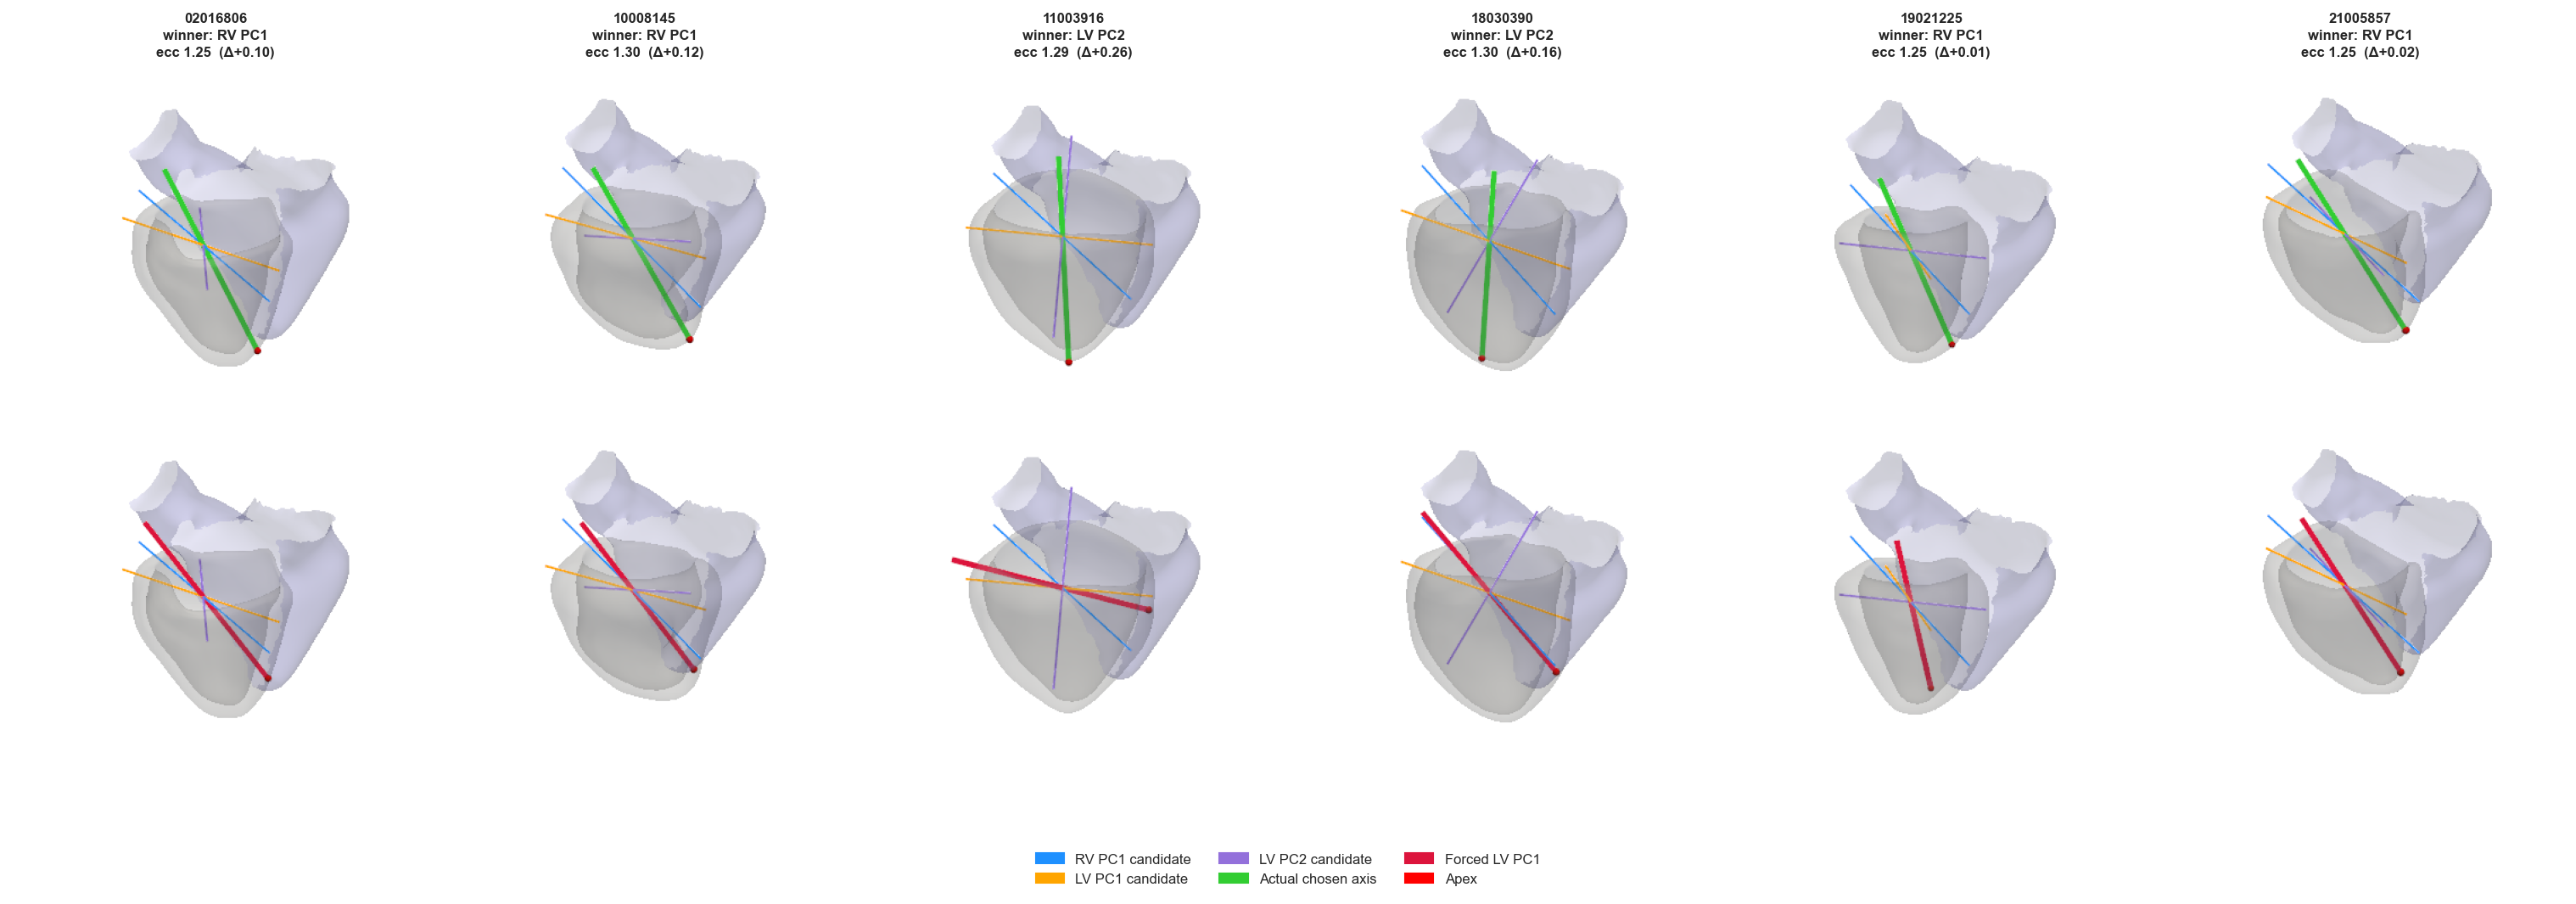
\includegraphics[width=\textwidth]{figures/fig2_axis_winner_vs_pc1}
    \caption{Per-patient comparison of apex-defining direction selected by the multi-candidate algorithm versus a forced LV~PC1 baseline. Cases where the algorithm selects RV~PC1 or LV~PC2 correspond to failures of the single-direction approach, visible as incorrect apex locations shifted toward the lateral wall or base. All 105 cases are shown.}
    \label{fig:app_axis_winner}
\end{figure}

\section{Implementation Details}
[Extended code descriptions, hyperparameter tables.]

\section{Dataset Details}
[Extended cohort statistics, data dictionary.]


\end{document}
